%%%%%%%%%%%%%%%%%%%%%%%%%%%%%%%%%%%%
% スライドオプション
%%%%%%%%%%%%%%%%%%%%%%%%%%%%%%%%%%%%

% オプション1：解答あり（授業用）

\documentclass[slidestop,compress,mathserif]{beamer}
\newcommand{\soln}[1]{\textit{#1}}
\newcommand{\solnGr}[1]{#1}

% オプション2：解答なし（配布用ハンドアウト）

%\documentclass[11pt,containsverbatim,handout]{beamer}
%\usepackage{pgfpages}
%\pgfpagesuselayout{4 on 1}[letterpaper,landscape,border shrink=5mm]
%\newcommand{\soln}[1]{ }
%\newcommand{\solnGr}{ }

%%%%%%%%%%%%%%%%%%%%%%%%%%%%%%%%%%%%
% 日本語サポート（LuaLaTeX使用）
% コンパイルコマンド: lualatex chp9.tex
%%%%%%%%%%%%%%%%%%%%%%%%%%%%%%%%%%%%

\usepackage{luatexja}
\usepackage{luatexja-fontspec}

%%%%%%%%%%%%%%%%%%%%%%%%%%%%%%%%%%%%
% スタイル
%%%%%%%%%%%%%%%%%%%%%%%%%%%%%%%%%%%%

\input{../lec_style_JP}

\setbeamertemplate{footline}{%
  \insertframenumber\,/\,\inserttotalframenumber}

%%%%%%%%%%%%%%%%%%%%%%%%%%%%%%%%%%%%
% プリアンブル
%%%%%%%%%%%%%%%%%%%%%%%%%%%%%%%%%%%%

\title[第9章：重回帰とロジスティック回帰]{第9章：重回帰とロジスティック回帰}
\author{OpenIntro Statistics 第4版（日本語版）}
\institute{$\:$ \\ {\footnotesize 原著スライド：Mine \c{C}etinkaya-Rundel（OpenIntro）\\
\webLink{http://creativecommons.org/licenses/by-sa/3.0/us/}{CC BY-SA ライセンス}のもと使用・翻訳。\\
一部の画像はフェアユース（教育目的）に基づき使用。}}
\date{}

%%%%%%%%%%%%%%%%%%%%%%%%%%%%%%%%%%%%
% ドキュメント開始
%%%%%%%%%%%%%%%%%%%%%%%%%%%%%%%%%%%%

\begin{document}


%%%%%%%%%%%%%%%%%%%%%%%%%%%%%%%%%%%%
% タイトルページ
%%%%%%%%%%%%%%%%%%%%%%%%%%%%%%%%%%%%

{
\addtocounter{framenumber}{-1}
{\removepagenumbers
\usebackgroundtemplate{
\includegraphics[width=\paperwidth]{../OpenIntro_Grid_4_3-01.jpg}}
\begin{frame}

\hfill 
\includegraphics[width=20mm]{../oiLogo_highres}

\titlepage

\end{frame}
}
}


%%%%%%%%%%%%%%%%%%%%%%%%%%%%%%%%%%%%
% 各節
%%%%%%%%%%%%%%%%%%%%%%%%%%%%%%%%%%%%

%%%%%%%%%%%%%%%%%%%%%%%%%%%%%%%%%%%%

\section{重回帰入門}

%%%%%%%%%%%%%%%%%%%%%%%%%%%%%%%%%%%%

\begin{frame}
\frametitle{重回帰}

\begin{itemize}

\item 単純線形回帰：2変数 --- 応答変数 $y$ と説明変数 $x$

\item 重線形回帰：複数変数 --- 応答変数 $y$ と説明変数 $x_1, x_2, \cdots$

\end{itemize}

\end{frame}

%%%%%%%%%%%%%%%%%%%%%%%%%%%%%%%%%%%%

\subsection{ダミー変数とカテゴリ変数を予測変数として用いる}

%%%%%%%%%%%%%%%%%%%%%%%%%%%%%%%%%%%

\begin{frame}
\frametitle{貧困率 vs. 地域（東部・西部）}


\[ \widehat{poverty} = 11.17 + 0.38 \times west \]

\begin{itemize}

\item 説明変数：地域、\hl{参照水準：}東部（east）

\item \hl{切片：}東部の州における貧困率の推定平均は 11.17\%
\begin{itemize}
\item 説明変数に \orange{0} を代入したときの値
\end{itemize}

\item \hl{傾き：}西部の州における貧困率の推定平均は東部より 0.38\% 高い。
\begin{itemize}
\item したがって、西部の州の貧困率の推定平均は 11.17 + 0.38 = 11.55\%。
\item 説明変数に \orange{1} を代入したときの値
\end{itemize}

\end{itemize}

\end{frame}

%%%%%%%%%%%%%%%%%%%%%%%%%%%%%%%%%%

\begin{frame}
\frametitle{貧困率 vs. 地域（北東部・中西部・西部・南部）}

\pq{北東部（northeast）・中西部（midwest）・西部（west）・南部（south）のうち、参照水準はどれか？}

{\small
\begin{center}
\begin{tabular}{rrrrr}
  \hline
 & Estimate & Std. Error & t value & Pr($>$$|$t$|$) \\
  \hline
(Intercept) & 9.50 & 0.87 & 10.94 & 0.00 \\
region4midwest & 0.03 & 1.15 & 0.02 & 0.98 \\
region4west & 1.79 & 1.13 & 1.59 & 0.12 \\
region4south & 4.16 & 1.07 & 3.87 & 0.00 \\
   \hline
\end{tabular}
\end{center}
}

\begin{enumerate}[(a)]
\solnMult{northeast（北東部）}
\item midwest（中西部）
\item west（西部）
\item south（南部）
\item 判別できない
\end{enumerate}

\end{frame}

%%%%%%%%%%%%%%%%%%%%%%%%%%%%%%%%%%%

\begin{frame}
\frametitle{貧困率 vs. 地域（北東部・中西部・西部・南部）}

\pq{北東部・中西部・西部・南部のうち、最も貧困率が低い地域はどれか？}

{\small
\begin{center}
\begin{tabular}{rrrrr}
  \hline
 & Estimate & Std. Error & t value & Pr($>$$|$t$|$) \\
  \hline
(Intercept) & 9.50 & 0.87 & 10.94 & 0.00 \\
region4midwest & 0.03 & 1.15 & 0.02 & 0.98 \\
region4west & 1.79 & 1.13 & 1.59 & 0.12 \\
region4south & 4.16 & 1.07 & 3.87 & 0.00 \\
   \hline
\end{tabular}
\end{center}
}

\begin{enumerate}[(a)]
\solnMult{northeast（北東部）}
\item midwest（中西部）
\item west（西部）
\item south（南部）
\item 判別できない
\end{enumerate}

\end{frame}

%%%%%%%%%%%%%%%%%%%%%%%%%%%%%%%%%%%%

\subsection{モデルへの多変数の組み込みと評価}

%%%%%%%%%%%%%%%%%%%%%%%%%%%%%%%%%%%%

\begin{frame}
\frametitle{本の重量}

\twocol{0.6}{0.4}{
{\footnotesize
\begin{center}
\begin{tabular}{rrrc}
  \hline
 & 重量 (g) & 体積 (cm$^\text{3}$) & カバー \\
  \hline
1 & 800 & 885 & hc \\
  2 & 950 & 1016 & hc \\
  3 & 1050 & 1125 & hc \\
  4 & 350 & 239 & hc \\
  5 & 750 & 701 & hc \\
  6 & 600 & 641 & hc \\
  7 & 1075 & 1228 & hc \\
  8 & 250 & 412 & pb \\
  9 & 700 & 953 & pb \\
  10 & 650 & 929 & pb \\
  11 & 975 & 1492 & pb \\
  12 & 350 & 419 & pb \\
  13 & 950 & 1010 & pb \\
  14 & 425 & 595 & pb \\
  15 & 725 & 1034 & pb \\
   \hline
\end{tabular}
\end{center}
}}
{
\begin{center}
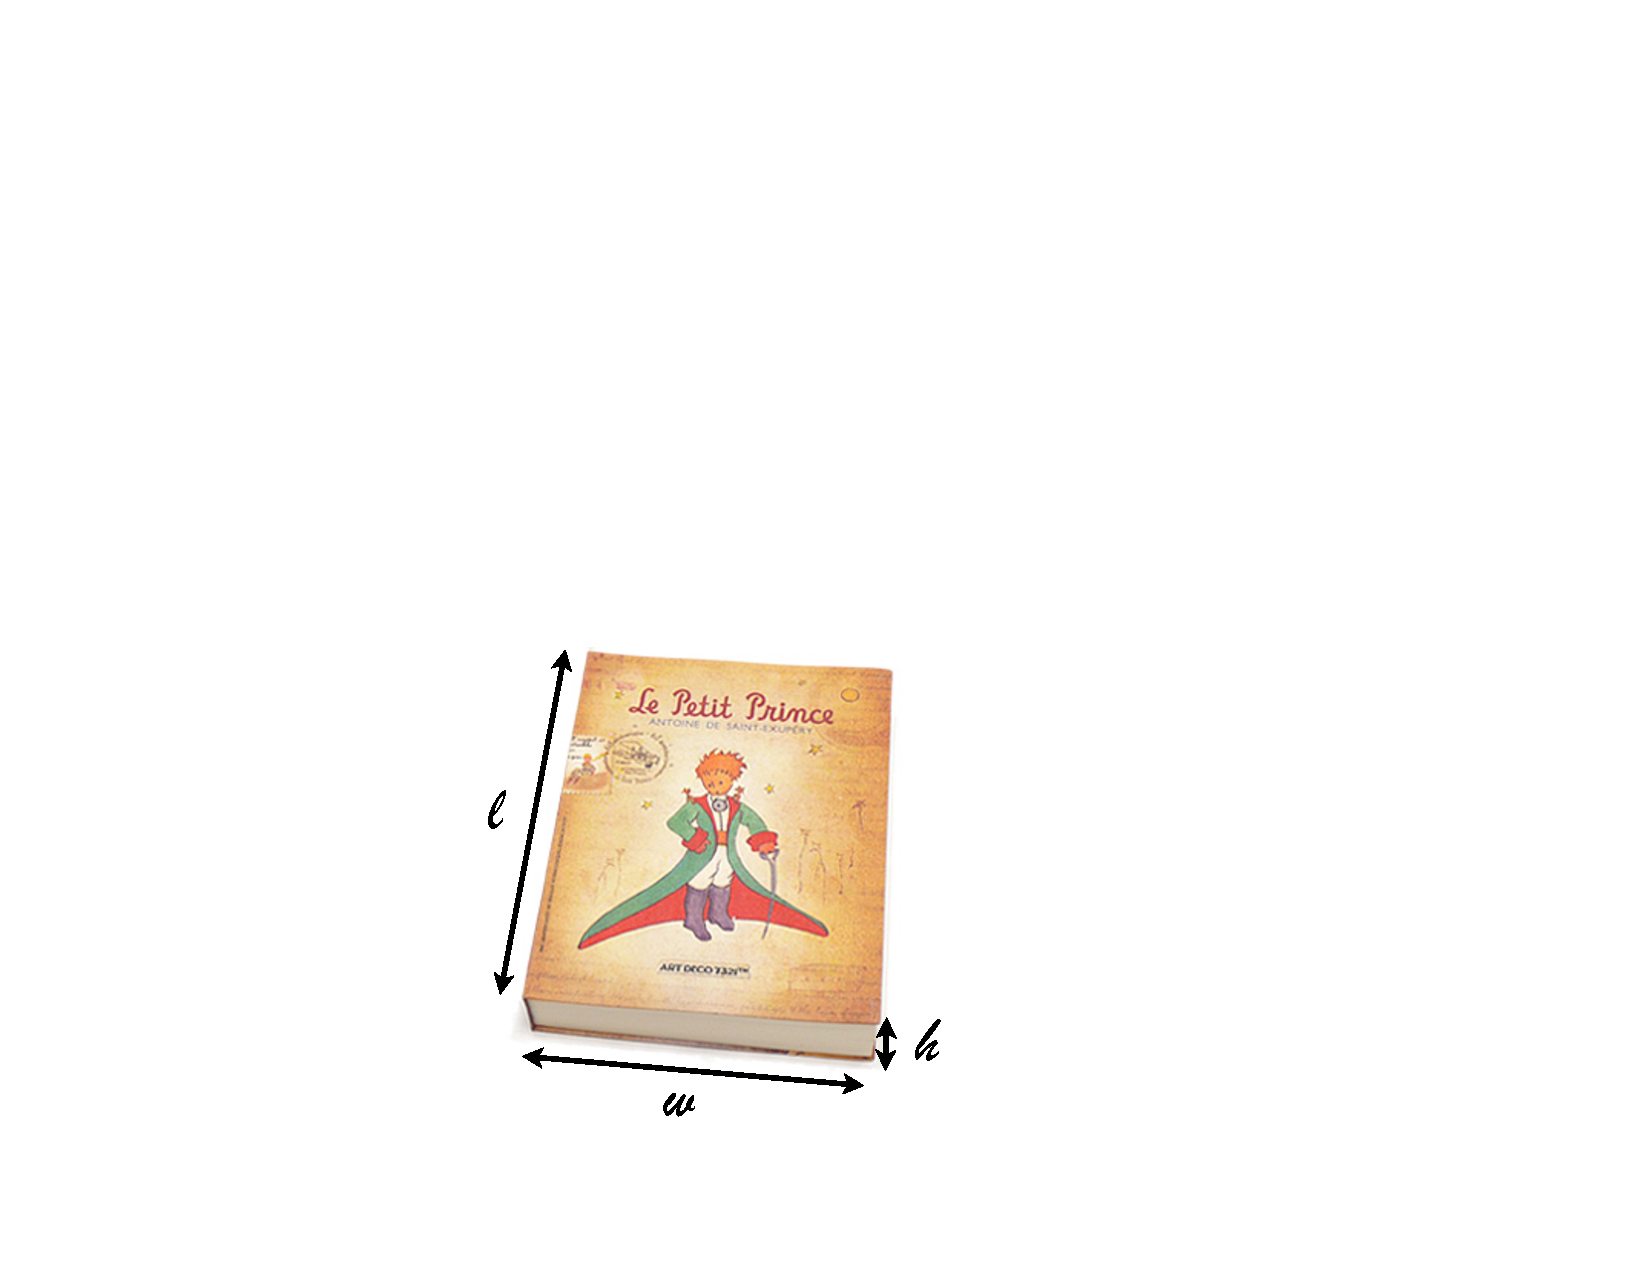
\includegraphics[width=0.7\textwidth]{9-1_intro_mlr/figures/books/book}
\end{center}
}

\ct{From: Maindonald, J.H. and Braun, W.J. (2nd ed., 2007) ``Data Analysis and Graphics Using R"}

\end{frame}

%%%%%%%%%%%%%%%%%%%%%%%%%%%%%%%%%%%

\begin{frame}
\frametitle{本の重量（続き）}

\twocol{0.45}{0.4}
{
\pq{{\small 散布図は本の重量と体積の関係、および回帰出力を示している。以下のうち正しいものはどれか？}}
}
{
\begin{center}
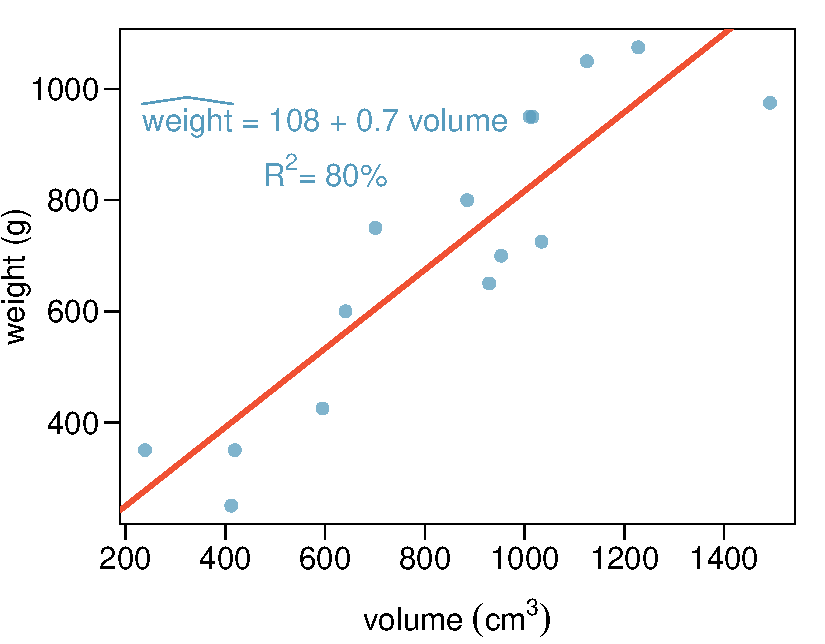
\includegraphics[width=\textwidth]{9-1_intro_mlr/figures/books/weight_volume}
\end{center}
}

\begin{enumerate}[(a)]
\item このモデルで本の 80\% の重量を正確に予測できる。
\solnMult{体積が平均より 10 cm$^\text{3}$ 大きい本は、重量が平均より約 7 g 重いと予測される。}
\item 重量と体積の相関係数は $R = 0.80^2 = 0.64$ である。
\item このモデルは最も体積の大きい本の重量を過小推定している。
\end{enumerate}

\end{frame}

%%%%%%%%%%%%%%%%%%%%%%%%%%%%%%%%%%%

\begin{frame}[fragile]
\frametitle{体積を用いた本の重量のモデリング}

{\small \textit{出力の一部を省略...}}

\begin{verbatim}
Coefficients:
             Estimate Std. Error t value Pr(>|t|)
(Intercept) 107.67931   88.37758   1.218    0.245
volume        0.70864    0.09746   7.271 6.26e-06


Residual standard error: 123.9 on 13 degrees of freedom
Multiple R-squared: 0.8026,	Adjusted R-squared: 0.7875
F-statistic: 52.87 on 1 and 13 DF,  p-value: 6.262e-06
\end{verbatim}

\end{frame}

%%%%%%%%%%%%%%%%%%%%%%%%%%%%%%%%%%%

\begin{frame}
\frametitle{ハードカバーとペーパーバックの重量}

\dq{ハードカバーとペーパーバックの体積と重量の関係において、何かトレンドを見つけられるか？}

\soln{{\small 体積を一定にした場合、ペーパーバックは一般的にハードカバーより軽い。}}

\begin{center}
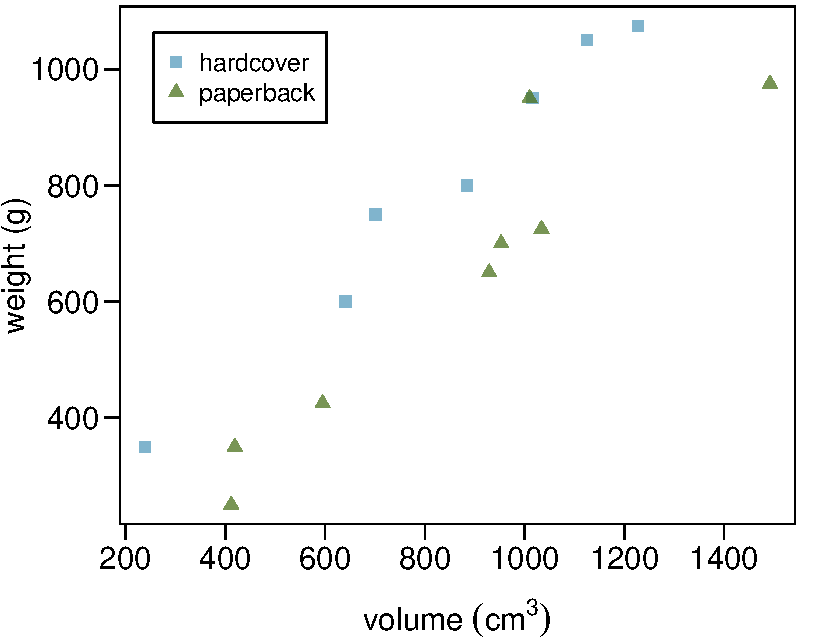
\includegraphics[width=0.6\textwidth]{9-1_intro_mlr/figures/books/weight_volume_cover}
\end{center}

\end{frame}

%%%%%%%%%%%%%%%%%%%%%%%%%%%%%%%%%%%

\begin{frame}[fragile]
\frametitle{体積\underline{とカバー種類}を用いた本の重量のモデリング}

\begin{verbatim}
Coefficients:
              Estimate Std. Error t value Pr(>|t|)
(Intercept)  197.96284   59.19274   3.344 0.005841 **
volume         0.71795    0.06153  11.669  6.6e-08 ***
cover:pb    -184.04727   40.49420  -4.545 0.000672 ***


Residual standard error: 78.2 on 12 degrees of freedom
Multiple R-squared: 0.9275,	Adjusted R-squared: 0.9154
F-statistic: 76.73 on 2 and 12 DF,  p-value: 1.455e-07
\end{verbatim}

\end{frame}

%%%%%%%%%%%%%%%%%%%%%%%%%%%%%%%%%%%

\begin{frame}
\frametitle{参照水準の決定}

\pq{以下の回帰出力に基づき、変数 \var{cover} の参照水準はどれか？なお \var{pb}：ペーパーバック。}

{\small
\begin{center}
\begin{tabular}{rrrrr}
  \hline
 & Estimate & Std. Error & t value & Pr($>$$|$t$|$) \\
  \hline
(Intercept) & 197.9628 & 59.1927 & 3.34 & 0.0058 \\
  volume & 0.7180 & 0.0615 & 11.67 & 0.0000 \\
  cover:pb & -184.0473 & 40.4942 & -4.55 & 0.0007 \\
   \hline
\end{tabular}
\end{center}
}

\begin{enumerate}[(a)]
\item ペーパーバック（paperback）
\solnMult{ハードカバー（hardcover）}
\end{enumerate}

\end{frame}

%%%%%%%%%%%%%%%%%%%%%%%%%%%%%%%%%%%

\begin{frame}
\frametitle{参照水準の決定}

\pq{以下のうち、この回帰モデルにおける変数の役割を正しく説明しているものはどれか？}

{\small
\begin{center}
\begin{tabular}{rrrrr}
  \hline
 & Estimate & Std. Error & t value & Pr($>$$|$t$|$) \\
  \hline
(Intercept) & 197.9628 & 59.1927 & 3.34 & 0.0058 \\
  volume & 0.7180 & 0.0615 & 11.67 & 0.0000 \\
  cover:pb & -184.0473 & 40.4942 & -4.55 & 0.0007 \\
   \hline
\end{tabular}
\end{center}
}

\begin{enumerate}[(a)]
\item 応答変数：重量、説明変数：体積、ペーパーバック
\item 応答変数：重量、説明変数：体積、ハードカバー
\item 応答変数：体積、説明変数：重量、カバー種類
\solnMult{応答変数：重量、説明変数：体積、カバー種類}
\end{enumerate}

\end{frame}

%%%%%%%%%%%%%%%%%%%%%%%%%%%%%%%%%%%

\begin{frame}
\frametitle{線形モデル}

{\small
\begin{center}
\begin{tabular}{rrrrr}
  \hline
 & Estimate & Std. Error & t value & Pr($>$$|$t$|$) \\
  \hline
(Intercept) & 197.96 & 59.19 & 3.34 & 0.01 \\
  volume & 0.72 & 0.06 & 11.67 & 0.00 \\
  cover:pb & -184.05 & 40.49 & -4.55 & 0.00 \\
   \hline
\end{tabular}
\end{center}
}

\[ \widehat{weight} = 197.96 + 0.72~volume - 184.05~cover:pb  \]

\begin{enumerate}

\item \hl{ハードカバー}の場合：\var{cover} に \orange{0} を代入
\begin{eqnarray*}
\widehat{weight} &=& 197.96 + 0.72~volume - 184.05 \times \orange{0} \\
&=& 197.96 +  0.72~volume
\end{eqnarray*}

\item \orange{ペーパーバック}の場合：\var{cover} に \orange{1} を代入
\begin{eqnarray*}
\widehat{weight} &=& 197.96 + 0.72~volume - 184.05 \times \orange{1} \\
&=& 13.91 +  0.72~volume
\end{eqnarray*}

\end{enumerate}

\end{frame}

%%%%%%%%%%%%%%%%%%%%%%%%%%%%%%%%%%%

\begin{frame}
\frametitle{線形モデルの可視化}

\begin{center}
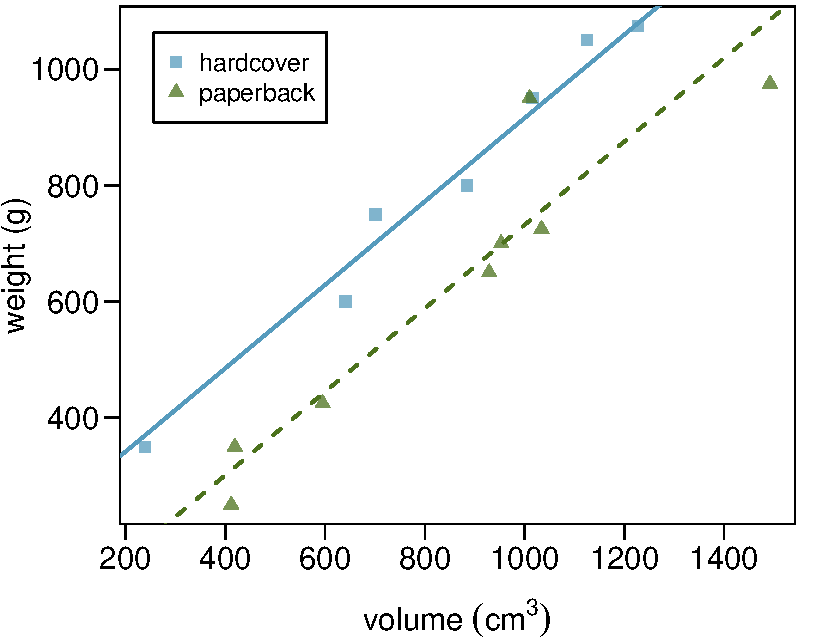
\includegraphics[width=0.8\textwidth]{9-1_intro_mlr/figures/books/weight_volume_cover_lines}
\end{center}

\end{frame}

%%%%%%%%%%%%%%%%%%%%%%%%%%%%%%%%%%%

\begin{frame}
\frametitle{回帰係数の解釈}

{\small
\begin{center}
\begin{tabular}{rrrrr}
  \hline
 & Estimate & Std. Error & t value & Pr($>$$|$t$|$) \\
  \hline
(Intercept) & 197.96 & 59.19 & 3.34 & 0.01 \\
  volume & 0.72 & 0.06 & 11.67 & 0.00 \\
  cover:pb & -184.05 & 40.49 & -4.55 & 0.00 \\
   \hline
\end{tabular}
\end{center}
}

\begin{itemize}

\item \hl{体積の傾き：}\underline{他の変数を一定に保つと}、体積が 1 cm$^3$ 大きい本は重量が約 0.72 g 重い傾向がある。

\item \hl{カバーの傾き：}\underline{他の変数を一定に保つと}、ペーパーバックはハードカバーより 184 g 軽いとモデルは予測する。

\item \hl{切片：}体積ゼロのハードカバーの平均重量は 198 g と予測される。
\begin{itemize}
\item 明らかに、この切片は文脈的に意味をなさない。直線の高さを調整するためだけのものである。
\end{itemize}

\end{itemize}

\end{frame}

%%%%%%%%%%%%%%%%%%%%%%%%%%%%%%%%%%%

\begin{frame}
\frametitle{予測}

\pq{体積が 600 cm$^3$ のペーパーバックの予測重量を求める正しい計算式はどれか？}

{\small
\begin{center}
\begin{tabular}{rrrrr}
  \hline
 & Estimate & Std. Error & t value & Pr($>$$|$t$|$) \\
  \hline
(Intercept) & 197.96 & 59.19 & 3.34 & 0.01 \\
  volume & 0.72 & 0.06 & 11.67 & 0.00 \\
  cover:pb & -184.05 & 40.49 & -4.55 & 0.00 \\
   \hline
\end{tabular}
\end{center}
}

\begin{enumerate}[(a)]
\solnMult{197.96 + 0.72 * 600 - 184.05 * 1} \only<2->{\orange{~$= 445.91$ グラム}}
\item 184.05 + 0.72 * 600 - 197.96 * 1
\item 197.96 + 0.72 * 600 - 184.05 * 0
\item 197.96 + 0.72 * 1 - 184.05 * 600
\end{enumerate}

\end{frame}

%%%%%%%%%%%%%%%%%%%%%%%%%%%%%%%%%%%

\begin{frame}
\frametitle{別の例：子供の認知テストスコアのモデリング}

3〜4歳の子供の認知テストスコアを母親の特徴で予測する。データは米国成人女性とその子供を対象とした調査（全国縦断的青年調査のサブサンプル）。

{\small
\begin{center}
\begin{tabular}{rrlrlr}
  \hline
 & kid\_score & mom\_hs & mom\_iq & mom\_work & mom\_age \\
  \hline
1 &  65 & yes & 121.12 & yes &  27 \\
  \vdots \\
  5 & 115 & yes & 92.75 & yes &  27 \\
  6 &  98 & no & 107.90 & no &  18 \\
  \vdots \\
  434 &  70 & yes & 91.25 & yes &  25 \\
   \hline
\end{tabular}
\end{center}
}

\vfill

{\tiny Gelman, Hill. \textit{Data Analysis Using Regression and Multilevel/Hierarchical Models}. (2007) Cambridge University Press.}

\end{frame}

%%%%%%%%%%%%%%%%%%%%%%%%%%%%%%%%%%%

\begin{frame}
\frametitle{傾きの解釈}

\dq{\underline{母親の IQ の傾き}の正しい解釈はどれか？}

{\small
\begin{center}
\begin{tabular}{rrrrr}
  \hline
 & Estimate & Std. Error & t value & Pr($>$$|$t$|$) \\
  \hline
(Intercept) & 19.59 & 9.22 & 2.13 & 0.03 \\
  mom\_hs:yes & 5.09 & 2.31 & 2.20 & 0.03 \\
  mom\_iq & 0.56 & 0.06 & 9.26 & 0.00 \\
  mom\_work:yes & 2.54 & 2.35 & 1.08 & 0.28 \\
  mom\_age & 0.22 & 0.33 & 0.66 & 0.51 \\
   \hline
\end{tabular}
\end{center}
}

$\:$ \\

\soln{他の変数を一定に保つと、母親の IQ が 1 点高い子供は平均的に 0.56 点高いスコアをとる傾向がある。}

\end{frame}

%%%%%%%%%%%%%%%%%%%%%%%%%%%%%%%%%%%

\begin{frame}
\frametitle{傾きの解釈}

\dq{\underline{切片}の正しい解釈はどれか？}

{\small
\begin{center}
\begin{tabular}{rrrrr}
  \hline
 & Estimate & Std. Error & t value & Pr($>$$|$t$|$) \\
  \hline
(Intercept) & 19.59 & 9.22 & 2.13 & 0.03 \\
  mom\_hs:yes & 5.09 & 2.31 & 2.20 & 0.03 \\
  mom\_iq & 0.56 & 0.06 & 9.26 & 0.00 \\
  mom\_work:yes & 2.54 & 2.35 & 1.08 & 0.28 \\
  mom\_age & 0.22 & 0.33 & 0.66 & 0.51 \\
   \hline
\end{tabular}
\end{center}
}

$\:$ \\

\soln{高校に行っておらず、子供の生後3年間に働いておらず、IQ が 0 で年齢が 0 歳の母親を持つ子供の平均スコアは 19.59 と推定される。この切片は文脈的に全く意味をなさない。}

\end{frame}

%%%%%%%%%%%%%%%%%%%%%%%%%%%%%%%%%%%

\begin{frame}
\frametitle{傾きの解釈}

\pq{\var{mom\_work} の傾きの正しい解釈はどれか？}

{\scriptsize
\begin{center}
\begin{tabular}{rrrrr}
  \hline
 & Estimate & Std. Error & t value & Pr($>$$|$t$|$) \\
  \hline
(Intercept) & 19.59 & 9.22 & 2.13 & 0.03 \\
  mom\_hs:yes & 5.09 & 2.31 & 2.20 & 0.03 \\
  mom\_iq & 0.56 & 0.06 & 9.26 & 0.00 \\
  mom\_work:yes & 2.54 & 2.35 & 1.08 & 0.28 \\
  mom\_age & 0.22 & 0.33 & 0.66 & 0.51 \\
   \hline
\end{tabular}
\end{center}
}

他の条件が等しい場合、子供の生後3年間に母親が働いていた子供は、働いていなかった子供と比べて
\begin{enumerate}[(a)]
\item スコアが 2.54 点低いと推定される
\solnMult{スコアが 2.54 点高いと推定される}
\end{enumerate}

\end{frame}

%%%%%%%%%%%%%%%%%%%%%%%%%%%%%%%%%%%

\subsection{重回帰のより良いツールとしての自由度調整済み $R^2$}

%%%%%%%%%%%%%%%%%%%%%%%%%%%%%%%%%%%

\begin{frame}
\frametitle{復習：貧困率のモデリング}

\vspace{-0.75cm}

\begin{center}
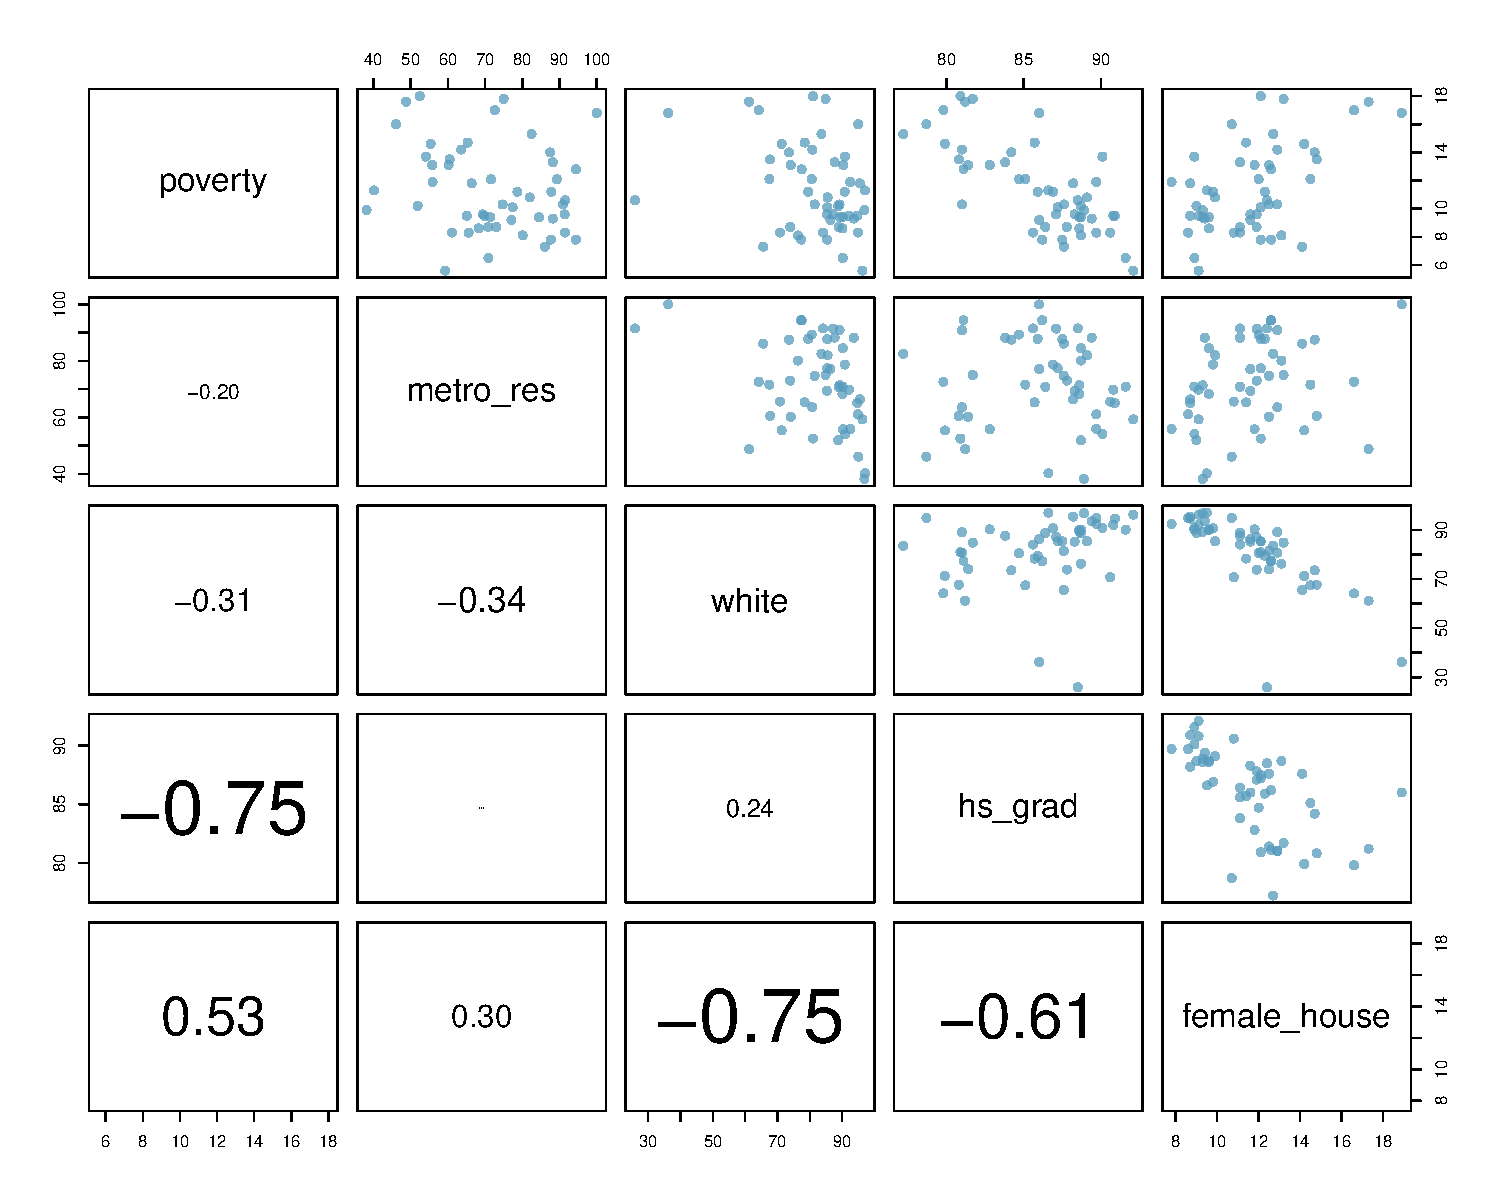
\includegraphics[width=0.9\textwidth]{9-1_intro_mlr/figures/poverty/poverty}
\end{center}

\end{frame}

%%%%%%%%%%%%%%%%%%%%%%%%%%%%%%%%%%%

\begin{frame}[fragile]
\frametitle{\% 女性世帯主を用いた貧困率の予測}

\vspace{-0.25cm}

\begin{center}
\begin{tabular}{rrrrr}
  \hline
 & Estimate & Std. Error & t value & Pr($>$$|$t$|$) \\
  \hline
(Intercept) & 3.31 & 1.90 & 1.74 & 0.09 \\
  female\_house & 0.69 & 0.16 & 4.32 & 0.00 \\
   \hline
\end{tabular}
\end{center}
\twocol{0.5}{0.4}
{
\begin{center}
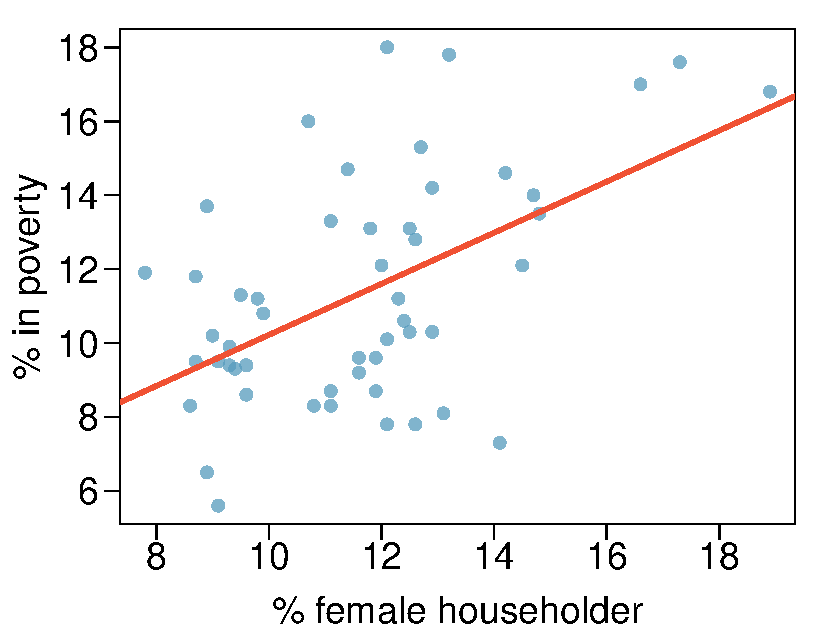
\includegraphics[width=\textwidth]{9-1_intro_mlr/figures/poverty/poverty_female_house}
\end{center}
}
{
\begin{align*}
R &= 0.53 \\
R^2 &= 0.53^2 = 0.28
\end{align*}
}

\end{frame}

%%%%%%%%%%%%%%%%%%%%%%%%%%%%%%%%%%%

\begin{frame}[fragile]
\frametitle{$R^2$ を改めて見る}

$R^2$ は3通りの方法で計算できる：

\begin{enumerate}

\item $x$ と $y$ の相関係数を2乗する {\small （これまでの計算方法）}

\item $y$ と $\hat{y}$ の相関係数を2乗する

\item 定義に基づいて計算する：

\[ R^2 = \frac{\text{$y$ の説明された変動}}{\text{$y$ の全変動}} \]

\end{enumerate}

\hl{分散分析（ANOVA）}を用いると、$y$ の説明された変動と全変動を計算できる。

\end{frame}


%%%%%%%%%%%%%%%%%%%%%%%%%%%%%%%%%%

\begin{frame}[fragile]
\frametitle{平方和}

\vspace{-0.5cm}

{\small
\begin{center}
\begin{tabular}{lrrrrr}
  \hline
 & Df & Sum Sq & Mean Sq & F value & Pr($>$F) \\
  \hline
female\_house & 1 & 132.57 & 132.57 & 18.68 & 0.00 \\
  Residuals & 49 & 347.68 & 7.10 &  &  \\
   \hline
Total & 50 & 480.25 \\
   \hline
\end{tabular}
\end{center}
}

\begin{changemargin}{-1cm}{-1cm}
\begin{eqnarray*}
\text{$y$ の平方和：} SS_{Total} &=& \sum(y - \bar{y})^2 = 480.25 \orange{ {\footnotesize ~$\rightarrow$ 全変動}} \\
\text{残差平方和：} SS_{Error} &=& \sum e_i^2 = 347.68 \orange{ { \footnotesize ~$\rightarrow$ 説明されていない変動}} \\
\text{$x$ の平方和：} SS_{Model} &=& SS_{Total} - SS_{Error} \orange{ {\footnotesize ~$\rightarrow$ 説明された変動}} \\
&=& 480.25 - 347.68 = 132.57
\end{eqnarray*}
\end{changemargin}

\[ R^2 = \frac{\text{説明された変動}}{\text{全変動}} = \frac{132.57}{480.25} = 0.28 \green{~$\checkmark$} \]

\end{frame}

%%%%%%%%%%%%%%%%%%%%%%%%%%%%%%%%%%

\begin{frame}
\frametitle{なぜ別の方法が必要か？}

\dq{相関係数の2乗として $R^2$ を計算する完全な方法があるのに、なぜ別のアプローチが必要なのか？}

\soln{\begin{itemize}
\item 単一予測変数の線形回帰では、同じ値を3通りで計算することはやりすぎに見えるかもしれない。
\item しかし、重線形回帰では $x$ が複数あるため、$x$ と $y$ の相関係数の2乗として $R^2$ を計算することができない。
\item 次に学ぶ \hl{自由度調整済み $R^2$} は説明された変動と説明されていない変動の比率という3番目のアプローチを必要とする。
\end{itemize}}

\end{frame}

%%%%%%%%%%%%%%%%%%%%%%%%%%%%%%%%%%

\begin{frame}
\frametitle{\% 女性世帯主 + \% 白人を用いた貧困率の予測}


\begin{center}
\begin{tabular}{rrrrr}
  \hline
\hl{線形モデル：}&  Estimate & Std. Error & t value & Pr($>$$|$t$|$) \\
  \hline
(Intercept) & -2.58 & 5.78 & -0.45 & 0.66 \\
  female\_house & 0.89 & 0.24 & 3.67 & 0.00 \\
  white & 0.04 & 0.04 & 1.08 & 0.29 \\
   \hline
\end{tabular}
\end{center}

\vspace{0.1cm}

\begin{center}
\begin{tabular}{lrrrrr}
  \hline
\hl{ANOVA：} & Df & Sum Sq & Mean Sq & F value & Pr($>$F) \\
  \hline
female\_house & 1 & 132.57 & 132.57 & 18.74 & 0.00 \\
  white & 1 & 8.21 & 8.21 & 1.16 & 0.29 \\
  Residuals & 48 & 339.47 & 7.07 &  &  \\
   \hline
Total & 50 &    480.25\\
   \hline
\end{tabular}
\end{center}

\[ R^2 = \frac{\text{説明された変動}}{\text{全変動}} = \frac{132.57 + 8.21}{480.25} = 0.29 \]

\end{frame}

%%%%%%%%%%%%%%%%%%%%%%%%%%%%%%%%%%%

\begin{frame}
\frametitle{}

\dq{変数 \var{white} をモデルに追加することで、\var{female\_house} が提供していなかった有益な情報が加わるか？}

\begin{center}
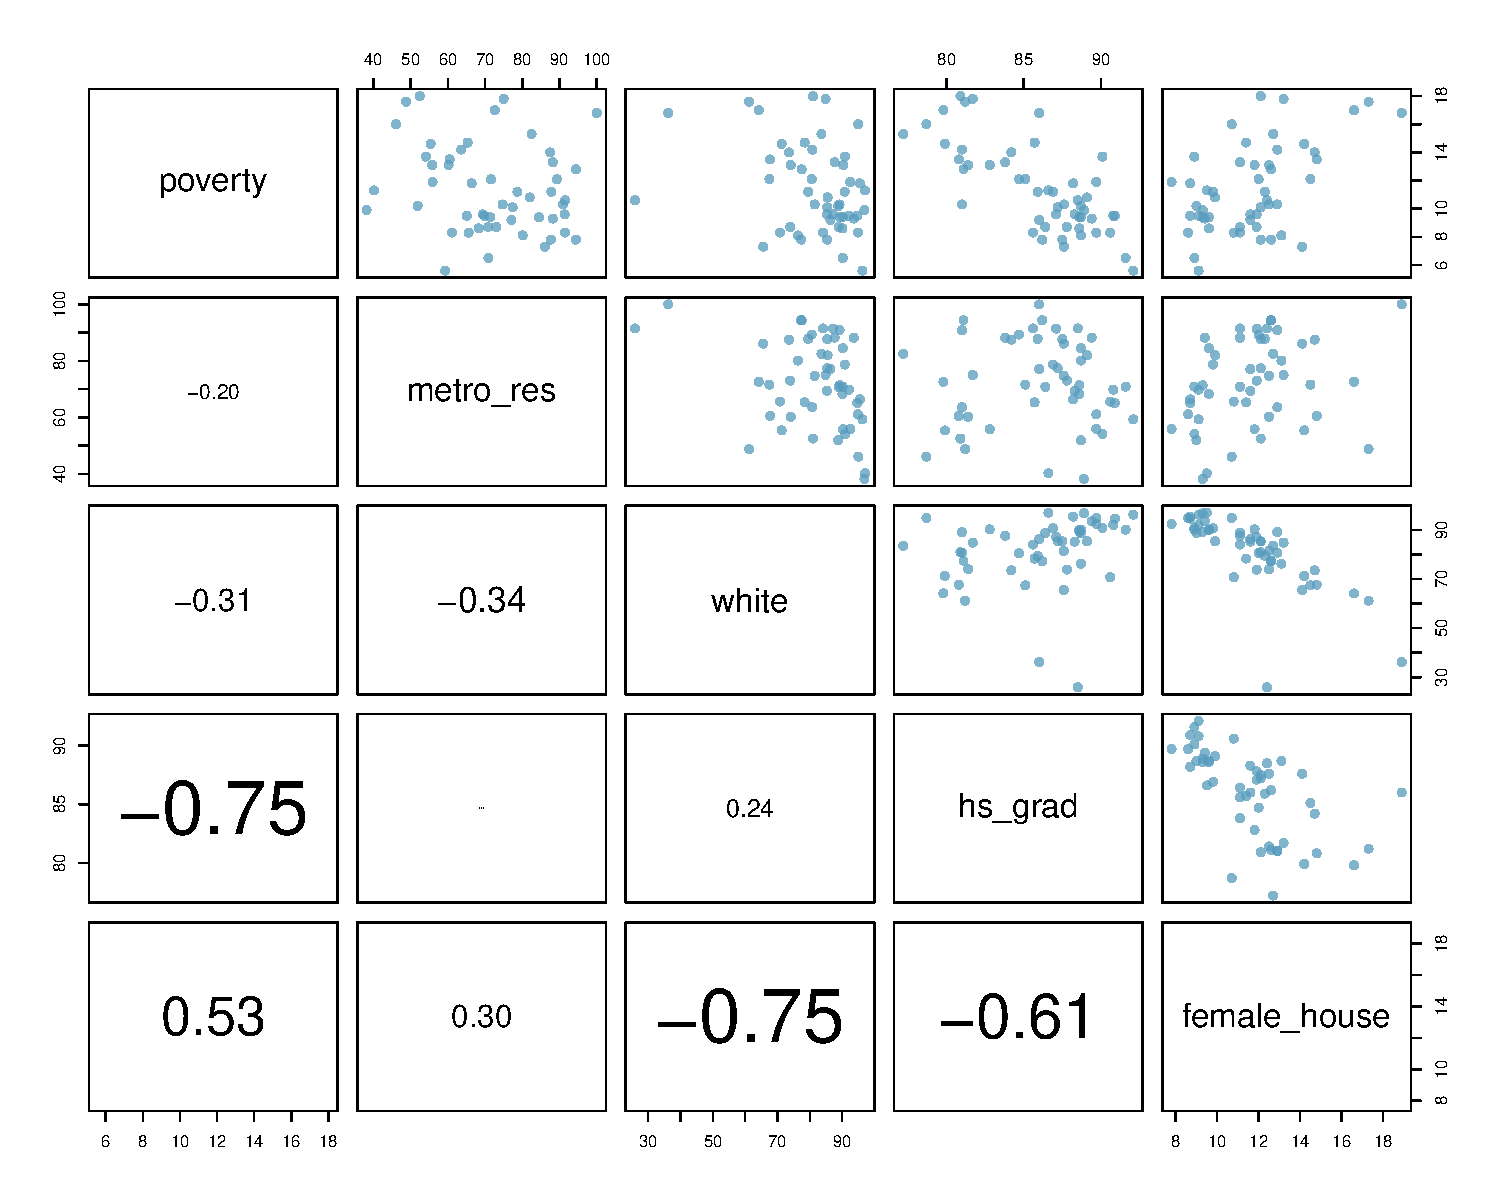
\includegraphics[width=0.8\textwidth]{9-1_intro_mlr/figures/poverty/poverty}
\end{center}

\end{frame}

%%%%%%%%%%%%%%%%%%%%%%%%%%%%%%%%%%%

\begin{frame}
\frametitle{説明変数間の多重共線性}

\hl{貧困率 vs. \% 女性世帯主}
\begin{center}
\begin{tabular}{rrrrr}
  \hline
 & Estimate & Std. Error & t value & Pr($>$$|$t$|$) \\
  \hline
(Intercept) & 3.31 & 1.90 & 1.74 & 0.09 \\
  female\_house & \orange{0.69} & 0.16 & 4.32 & 0.00 \\
   \hline
\end{tabular}
\end{center}

$\:$ \\

\hl{貧困率 vs. \% 女性世帯主 と \% 白人}
\begin{center}
\begin{tabular}{rrrrr}
  \hline
 & Estimate & Std. Error & t value & Pr($>$$|$t$|$) \\
  \hline
(Intercept) & -2.58 & 5.78 & -0.45 & 0.66 \\
  female\_house & \orange{0.89} & 0.24 & 3.67 & 0.00 \\
  white & 0.04 & 0.04 & 1.08 & 0.29 \\
   \hline
\end{tabular}
\end{center}

\end{frame}

%%%%%%%%%%%%%%%%%%%%%%%%%%%%%%%%%%%

\begin{frame}
\frametitle{説明変数間の多重共線性（続き）}

\begin{itemize}

\item 2つの予測変数が相関しているとき、それらは共線性があると言い、この\hl{多重共線性}はモデルの推定を複雑にする。\\
\Remember{予測変数は説明変数あるいは\underline{独立}変数とも呼ばれる。理想的には互いに独立であるべきである。}

\item 互いに関連した予測変数をモデルに加えることは好ましくない。そのような変数を追加しても、多くの場合何も得られないからである。代わりに、最もシンプルで優れたモデル、すなわち\hl{簡潔な（節約的な）}モデルを目指す。

\item 観測データから生じる多重共線性を完全に避けることは不可能だが、実験は通常、予測変数間の相関を防ぐように設計される。

\end{itemize}

\end{frame}

%%%%%%%%%%%%%%%%%%%%%%%%%%%%%%%%%%%

\begin{frame}[fragile]
\frametitle{$R^2$ vs. 自由度調整済み $R^2$}

\renewcommand\arraystretch{1.25}
\begin{center}
\begin{tabular}{l | c  c}
			& $R^2$	& 自由度調整済み $R^2$ \\
\hline
モデル1（単一予測変数）	& 0.28	& 0.26 \\
モデル2（重回帰）			& 0.29	& 0.26
\end{tabular}
\end{center}

\begin{itemize}

\item \underline{どんな}変数をモデルに加えても $R^2$ は増加する。

\item しかし、加えた変数が実際に新しい情報を提供しない場合や全く無関係な場合、自由度調整済み $R^2$ は増加しない。

\end{itemize}



\end{frame}

%%%%%%%%%%%%%%%%%%%%%%%%%%%%%%%%%%%

\begin{frame}
\frametitle{自由度調整済み $R^2$}

\formula{自由度調整済み $R^2$}
{\[ R^2_{adj} = 1 - \pr{ \frac{ SS_{Error} }{ SS_{Total} } \times \frac{n - 1}{n - p - 1} } \]
ここで $n$ はケース数、$p$ はモデル内の予測変数（説明変数）の数。
}

\begin{itemize}

\item $p$ が負になることはないため、$R^2_{adj}$ は常に $R^2$ より小さい。

\item $R^2_{adj}$ はモデルに含まれる予測変数の数に対してペナルティを課す。

\item したがって、$R^2_{adj}$ が高いモデルをより好ましいモデルとして選ぶ。

\end{itemize}

\end{frame}

%%%%%%%%%%%%%%%%%%%%%%%%%%%%%%%%%%%

\begin{frame}
\frametitle{自由度調整済み $R^2$ の計算}

\begin{center}
\begin{tabular}{lrrrrr}
  \hline
\hl{ANOVA：} & Df & Sum Sq & Mean Sq & F value & Pr($>$F) \\
  \hline
female\_house & 1 & 132.57 & 132.57 & 18.74 & 0.0001 \\
  white & 1 & 8.21 & 8.21 & 1.16 & 0.2868 \\
  Residuals & 48 & 339.47 & 7.07 &  &  \\
   \hline
Total & 50 &    480.25\\
   \hline
\end{tabular}
\end{center}

\begin{eqnarray*}
R^2_{adj} &=& 1 - \pr{ \frac{ SS_{Error} }{ SS_{Total} } \times \frac{n - 1}{n - p - 1} } \\
&=& 1 - \pr{ \frac{ 339.47 }{ 480.25 } \times \frac{51 - 1}{51 - 2 - 1} }   \\
&=& 1- \pr{ \frac{ 339.47 }{ 480.25 } \times \frac{50}{48} } \\
&=& 1 -  0.74 \\
&=& 0.26
\end{eqnarray*}

\end{frame}

%%%%%%%%%%%%%%%%%%%%%%%%%%%%%%%%%%%%

\section{モデル選択}

%%%%%%%%%%%%%%%%%%%%%%%%%%%%%%%%%%%%

\subsection{モデル内で有益でない可能性のある変数の識別}

%%%%%%%%%%%%%%%%%%%%%%%%%%%%%%%%%%%

\begin{frame}
\frametitle{教室における美貌}

\begin{itemize}

\item データ：テキサス大学の 463 コースにおける教員の美貌と授業評価の学生評価。

\item 評価は学期末に実施され、美貌の判定はその後、授業に参加しておらず授業評価を知らない 6 人の学生（上位学年の女性 2 人、男性 2 人、下位学年の女性 1 人、男性 1 人）が行った。

\end{itemize}

\ct{Hamermesh \& Parker. (2004)``Beauty in the classroom: instructors? pulchritude and putative pedagogical productivity? Economics Education Review.}

\end{frame}

%%%%%%%%%%%%%%%%%%%%%%%%%%%%%%%%%%%

\begin{frame}
\frametitle{教員評価 vs. 美貌}

教員評価スコア（高いほど良い）vs. 美貌スコア（0 が平均、負が平均以下、正が平均以上）：

\begin{center}
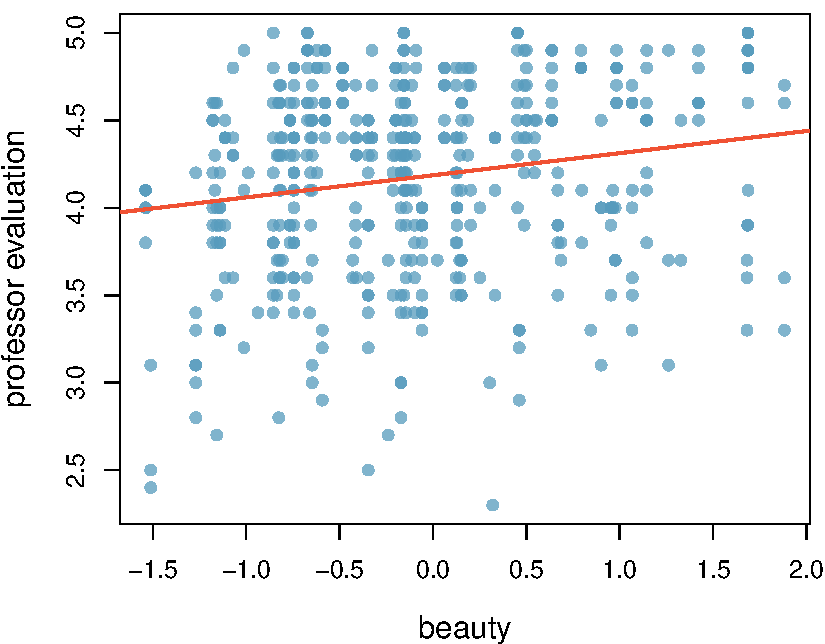
\includegraphics[width=0.65\textwidth]{9-2_model_select/figures/beauty/beauty_profeval}
\end{center}

\end{frame}

%%%%%%%%%%%%%%%%%%%%%%%%%%%%%%%%%%%

\begin{frame}
\frametitle{}

\pq{モデル出力に基づき、以下のうち\underline{正しい}ものはどれか？}

\begin{center}
{\small
\begin{tabular}{rrrrr}
  \hline
 & Estimate & Std. Error & t value & Pr($>$$|$t$|$) \\
  \hline
(Intercept) & 4.19 & 0.03 & 167.24 & 0.00 \\
  beauty & 0.13 & 0.03 & 4.00 & 0.00 \\
   \hline
$R^2$ = 0.0336
\end{tabular}
}
\end{center}

\begin{enumerate}[(a)]
\item このモデルは教員評価の 3.36\% を正確に予測できる。
\item 美貌は教員評価の有意な予測変数ではない。
\solnMult{美貌スコアが平均より 1 点高い教員は、評価も 0.13 点高い傾向がある。}
\item 美貌スコアの変動の 3.36\% は教員評価で説明できる。
\item 相関係数は $\sqrt{0.0336} = 0.18$ または $-0.18$ の可能性があるが、どちらか判別できない。
\end{enumerate}

\end{frame}

%%%%%%%%%%%%%%%%%%%%%%%%%%%%%%%%%%%

\begin{frame}
\frametitle{探索的分析}

\twocol{0.4}{0.6}
{
\dq{興味深い特徴はあるか？}
\soln{美貌スコアが非常に低い女性教員が少ない。}
$\:$ \\
\dq{同じ美貌スコアを持つ場合、男性教員は女性教員より高く評価されるか、低く評価されるか、ほぼ同じか？}
\soln{このプロットだけでは判断が難しい。}
}
{
\begin{center}
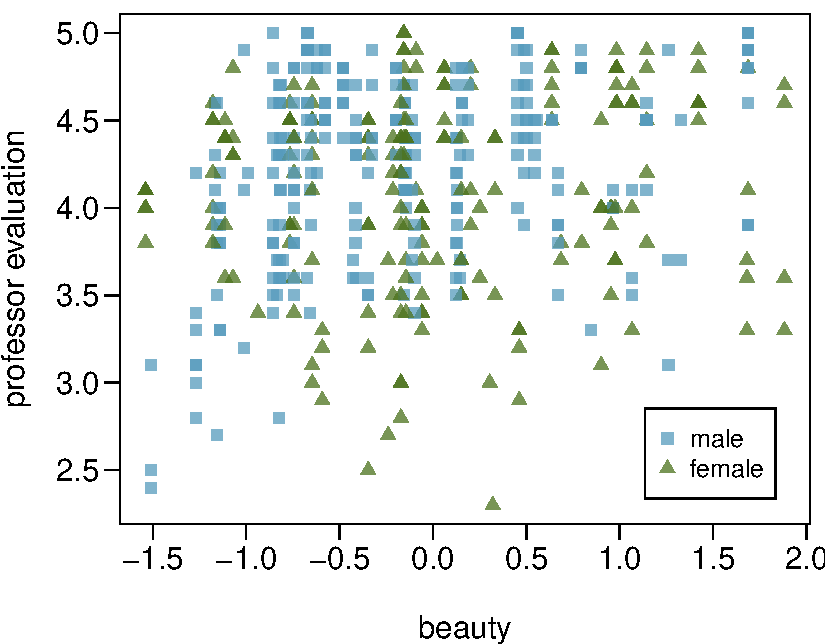
\includegraphics[width=\textwidth]{9-2_model_select/figures/beauty/beauty_profeval_gender}
\end{center}
}

\end{frame}

%%%%%%%%%%%%%%%%%%%%%%%%%%%%%%%%%%

\begin{frame}[fragile]
\frametitle{教員評価 vs. 美貌 + 性別}

\pq{同じ美貌スコアを持つ場合、男性教員は女性教員より高く評価されるか、低く評価されるか、ほぼ同じか？}

{\small
\begin{center}
\begin{tabular}{rrrrr}
  \hline
 & Estimate & Std. Error & t value & Pr($>$$|$t$|$) \\
  \hline
(Intercept) & 4.09 & 0.04 & 107.85 & 0.00 \\
  beauty & 0.14 & 0.03 & 4.44 & 0.00 \\
  gender.male & 0.17 & 0.05 & 3.38 & 0.00 \\
   \hline
$R^2_{adj}$ = 0.057
\end{tabular}
\end{center}
}

\begin{enumerate}[(a)]
\solnMult{高い} \only<2->{\orange{$\rightarrow$ 美貌を一定にすると、男性教員は女性教員より平均 0.17 点高く評価される。}}
\item 低い
\item ほぼ同じ
\end{enumerate}

\end{frame}

%%%%%%%%%%%%%%%%%%%%%%%%%%%%%%%%%%%

\begin{frame}[fragile]
\frametitle{フルモデル}

{\small
\begin{center}
\begin{tabular}{rrrrr}
  \hline
 & Estimate & Std. Error & t value & Pr($>$$|$t$|$) \\
  \hline
(Intercept) & 4.6282 & 0.1720 & 26.90 & 0.00 \\
  beauty & 0.1080 & 0.0329 & 3.28 & 0.00 \\
  gender.male & 0.2040 & 0.0528 & 3.87 & 0.00 \\
  age & -0.0089 & 0.0032 & -2.75 & 0.01 \\
formal.yes \footnote{\texttt{formal}：ネクタイ・ジャケット/ブラウスを着た写真、水準：\texttt{yes}、\texttt{no}} & 0.1511 & 0.0749 & 2.02 & 0.04 \\
  lower.yes \footnote{\texttt{lower}：下位学年のコース、水準：\texttt{yes}、\texttt{no}} & 0.0582 & 0.0553 & 1.05 & 0.29 \\
  native.non english & -0.2158 & 0.1147 & -1.88 & 0.06 \\
  minority.yes & -0.0707 & 0.0763 & -0.93 & 0.35 \\
  students \footnote{\texttt{students}：学生数} & -0.0004 & 0.0004 & -1.03 & 0.30 \\
  tenure.tenure track \footnote{\texttt{tenure}：テニュア状況、水準：\texttt{non-tenure track}、\texttt{tenure track}、\texttt{tenured}} & -0.1933 & 0.0847 & -2.28 & 0.02 \\
  tenure.tenured & -0.1574 & 0.0656 & -2.40 & 0.02 \\
   \hline
\end{tabular}
\end{center}
}

\end{frame}

%%%%%%%%%%%%%%%%%%%%%%%%%%%%%%%%%%%

\begin{frame}
\frametitle{仮説}

傾きパラメータの解釈がモデル内の他の変数を考慮に入れるように、予測変数の有意性をテストするための仮説も他の変数を考慮に入れる。

$\:$ \\

\begin{itemize}
\item[] \mathhl{H_0:} 他の説明変数がモデルに含まれるとき、$B_i = 0$。
\item[] \mathhl{H_A:} 他の説明変数がモデルに含まれるとき、$B_i \ne 0$。
\end{itemize}

\end{frame}

%%%%%%%%%%%%%%%%%%%%%%%%%%%%%%%%%%%

\begin{frame}
\frametitle{有意性の評価：数値変数}

\pq{年齢の p 値が 0.01 である。これは何を意味するか？}

{\scriptsize
\begin{center}
\begin{tabular}{rrrrr}
  \hline
 & Estimate & Std. Error & t value & Pr($>$$|$t$|$) \\
  \hline
...\\
  age & -0.0089 & 0.0032 & -2.75 & 0.01 \\
...\\
   \hline
\end{tabular}
\end{center}
}

\begin{enumerate}[(a)]
\item p 値が正なので、教員の年齢が高いほど評価も高いと予測される。
\solnMult{他の変数をモデルに保ったとき、教員の年齢が評価と関連しているという強い証拠がある。}
\item 年齢の真の傾きパラメータが 0 である確率は 0.01 である。
\item 年齢の真の傾きパラメータが -0.0089 である確率が約 1\% ある。
\end{enumerate}

\end{frame}

%%%%%%%%%%%%%%%%%%%%%%%%%%%%%%%%%%%

\begin{frame}[fragile]
\frametitle{有意性の評価：カテゴリ変数}

\pq{{\small テニュアは 3 水準のカテゴリ変数（non tenure track、tenure track、tenured）である。以下のモデル出力に基づき、\underline{誤り}はどれか？}}

{\footnotesize
\begin{center}
\begin{tabular}{rrrrr}
  \hline
 & Estimate & Std. Error & t value & Pr($>$$|$t$|$) \\
  \hline
... \\
  tenure.tenure track & -0.1933 & 0.0847 & -2.28 & 0.02 \\
  tenure.tenured & -0.1574 & 0.0656 & -2.40 & 0.02 \\
   \hline
\end{tabular}
\end{center}
}

\begin{enumerate}[(a)]
\item 参照水準は non tenure track である。
\item 他の条件が等しい場合、tenure track の教員は non-tenure track の教員より平均 0.19 点低く評価される。
\item 他の条件が等しい場合、tenured の教員は non-tenure track の教員より平均 0.16 点低く評価される。
\solnMult{他の条件が等しい場合、tenure track と tenured の教員の平均評価には有意な差がある。}
\end{enumerate}

\end{frame}

%%%%%%%%%%%%%%%%%%%%%%%%%%%%%%%%%%%

\begin{frame}
\frametitle{有意性の評価}

\dq{教員の評価スコアの有意な予測変数ではない可能性があるなど、モデルへの貢献が少ないと思われる予測変数はどれか？}

{\scriptsize
\begin{center}
\begin{tabular}{rrrrr}
  \hline
 & Estimate & Std. Error & t value & Pr($>$$|$t$|$) \\
  \hline
(Intercept) & 4.6282 & 0.1720 & 26.90 & 0.00 \\
  beauty & 0.1080 & 0.0329 & 3.28 & 0.00 \\
  gender.male & 0.2040 & 0.0528 & 3.87 & 0.00 \\
  age & -0.0089 & 0.0032 & -2.75 & 0.01 \\
  formal.yes & 0.1511 & 0.0749 & 2.02 & 0.04 \\
  \rowcolor{oiB!50}
  lower.yes & 0.0582 & 0.0553 & 1.05 & 0.29 \\
    \rowcolor{oiB!50}
  native.non english & -0.2158 & 0.1147 & -1.88 & 0.06 \\
    \rowcolor{oiB!50}
  minority.yes & -0.0707 & 0.0763 & -0.93 & 0.35 \\
    \rowcolor{oiB!50}
  students & -0.0004 & 0.0004 & -1.03 & 0.30 \\
  tenure.tenure track & -0.1933 & 0.0847 & -2.28 & 0.02 \\
  tenure.tenured & -0.1574 & 0.0656 & -2.40 & 0.02 \\
   \hline
\end{tabular}
\end{center}
}

\end{frame}

%%%%%%%%%%%%%%%%%%%%%%%%%%%%%%%%%%%

\subsection{2つのモデル選択戦略}

%%%%%%%%%%%%%%%%%%%%%%%%%%%%%%%%%%%

\begin{frame}
\frametitle{モデル選択戦略}

\dq{これまでに学んだことを踏まえ、どの変数をモデルに保ち、どれを除くかを決めるために使える方法をいくつか考えてみよ。}

\end{frame}


%%%%%%%%%%%%%%%%%%%%%%%%%%%%%%%%%%%

\begin{frame}
\frametitle{後退消去法}

\begin{enumerate}

\item フルモデルから始める
\item 1つの変数を除いて各小モデルの $R^2_{adj}$ を記録する
\item $R^2_{adj}$ が最も大きく増加したモデルを選ぶ
\item いずれのモデルも $R^2_{adj}$ が増加しなくなるまで繰り返す

\end{enumerate}

\end{frame}

%%%%%%%%%%%%%%%%%%%%%%%%%%%%%%%%%%%

\begin{frame}[shrink]
\frametitle{後退消去法}

\vspace{-0.3cm}

{\tiny
\begin{tabular}{l | l | c}
フル		& beauty + gender + age + formal + lower + native + minority + students + tenure & \orange{0.0839} \\
\hline
ステップ1 	& gender + age + formal + lower + native + minority + students + tenure		& 0.0642 \\
		& beauty + age + formal + lower + native + minority + students + tenure		& 0.0557 \\
		& beauty + gender + formal + lower + native + minority + students + tenure	& 0.0706 \\
		& beauty + gender + age + lower + native + minority + students + tenure		& 0.0777 \\
		& beauty + gender + age + formal + native + minority + students + tenure		& 0.0837 \\
		& beauty + gender + age + formal + lower + minority + students + tenure		& 0.0788 \\
		& beauty + gender + age + formal + lower + native + students + tenure		& \orange{0.0842} \\
		& beauty + gender + age + formal + lower + native + minority + tenure		& 0.0838 \\
		& beauty + gender + age + formal + lower + native + minority + students		& 0.0733 \\
\hline
ステップ2	& gender + age + formal + lower + native + students + tenure 				& 0.0647 \\
		& beauty + age + formal + lower + native + students + tenure 				& 0.0543 \\
		& beauty + gender + formal + lower + native + students + tenure 			& 0.0708 \\
		& beauty + gender + age + lower + native + students + tenure 				&0.0776  \\
		& beauty + gender + age + formal + native + students + tenure 			& \orange{0.0846} \\
		& beauty + gender + age + formal + lower + native + tenure 				& 0.0844 \\
		& beauty + gender + age + formal + lower + native + students 				& 0.0725 \\
\hline
ステップ3	& gender + age + formal + native + students + tenure 					& 0.0653 \\
		& beauty + age + formal + native + students + tenure					& 0.0534 \\
		& beauty + gender + formal + native + students + tenure					& 0.0707 \\
		& beauty + gender + age + native + students + tenure					& 0.0786 \\
		& beauty + gender + age + formal + students + tenure					& 0.0756 \\
		& beauty + gender + age + formal + native + tenure						& \orange{0.0855} \\
		& beauty + gender + age + formal + native + students					& 0.0713 \\
\hline
ステップ4	& gender + age + formal + native + tenure 							& 0.0667 \\
		& beauty + age + formal + native + tenure								& 0.0553 \\
		& beauty + gender + formal + native + tenure							& 0.0723 \\
		& beauty + gender + age + native + tenure							& 0.0806 \\
		& beauty + gender + age + formal + tenure							& 0.0773 \\
		& beauty + gender + age + formal + native							& 0.0713 \\
\end{tabular}
}

\end{frame}

%%%%%%%%%%%%%%%%%%%%%%%%%%%%%%%%%%%

\begin{frame}[fragile]
\frametitle{R の \texttt{step} 関数}

R の \texttt{step} 関数は同様の後退消去プロセスを行うが、
モデル選択に $R^2_{adj}$ の代わりに AIC（赤池情報量基準）という
異なる指標を使用する。

{\tiny
\begin{verbatim}
Call:
lm(formula = profevaluation ~ beauty + gender + age + formal +
    native + tenure, data = d)

Coefficients:
       (Intercept)              beauty          gendermale
          4.628435            0.105546            0.208079
               age           formalyes   nativenon english
         -0.008844            0.132422           -0.243003
tenuretenure track       tenuretenured
         -0.206784           -0.175967
\end{verbatim}
}

最良モデル：beauty + gender + age + formal + native + tenure

\end{frame}

%%%%%%%%%%%%%%%%%%%%%%%%%%%%%%%%%%%

\begin{frame}
\frametitle{前進選択法}

\begin{enumerate}

\item 応答変数 vs. 各説明変数の回帰から始める
\item $R^2_{adj}$ が最も高いモデルを選ぶ
\item 残りの変数を1つずつ既存のモデルに追加し、$R^2_{adj}$ が最も高いモデルを選ぶ
\item 残りの変数を追加しても $R^2_{adj}$ が増加しなくなるまで繰り返す

\end{enumerate}

\end{frame}

%%%%%%%%%%%%%%%%%%%%%%%%%%%%%%%%%%%

\subsection{自由度調整済み $R^2$ の代替としての p 値アプローチ}

%%%%%%%%%%%%%%%%%%%%%%%%%%%%%%%%%%%

\begin{frame}
\subsection{後退消去法と前進選択法}

\begin{itemize}

\item p 値アプローチによる後退消去法：
\begin{enumerate}
\item フルモデルから始める
\item p 値が最も高い変数を除いて小さいモデルを再適合する
\item モデルに残っているすべての変数が有意になるまで繰り返す
\end{enumerate}

\item p 値アプローチによる前進選択法：
\begin{enumerate}
\item 応答変数 vs. 各説明変数の回帰から始める
\item 最も低い有意な p 値を持つ変数を選ぶ
\item 残りの変数を1つずつ既存のモデルに追加し、最も低い有意な p 値を持つ変数を選ぶ
\item 残りの変数が有意な p 値を持たなくなるまで繰り返す
\end{enumerate}

\end{itemize}

\end{frame}

%%%%%%%%%%%%%%%%%%%%%%%%%%%%%%%%%%%

\begin{frame}
\frametitle{後退消去法：p 値アプローチ}

\resizebox{\textwidth}{!}{%
{\tiny
\begin{tabular}{l | rrrrrrrrrr }
\textbf{ステップ}		& \multicolumn{10}{c}{ \textbf{含まれる変数とp値} } \\
\hline
フル		& beauty	& gender		& age	& formal		& lower 	& native	 	& minority		& students	& tenure		& tenure \\
		& 		& male		& 		& yes		& yes	 & nonenglish	& yes		& 			& tenure track	& tenured \\
		&  0.00 	&  0.00 		& 0.01	& 0.04		& 0.29	& 0.06		& \orange{0.35}	& 0.30		& 0.02		& 0.02 \\
\hline
ステップ1	& beauty	& gender		& age	& formal		& lower 		& native	 	& 			& students	& tenure		& tenure \\
		& 		& male		& 		& yes		& yes		& nonenglish	& 			& 			& tenure track	& tenured \\
		&  0.00 	&  0.00 		& 0.01	& 0.04		& \orange{0.38}	& 0.03		&			& 0.34		& 0.02		& 0.01 \\
\hline
ステップ2	& beauty	& gender		& age	& formal		& 	 		& native	 	& 			& students	& tenure		& tenure \\
		& 		& male		& 		& yes		& 			& nonenglish	& 			& 			& tenure track	& tenured \\
		&  0.00 	&  0.00 		& 0.01	& 0.05		& 			& 0.02		&			& \orange{0.44}	& 0.01		& 0.01 \\
\hline
ステップ3 	& beauty	& gender		& age	& formal		& 	 		& native	 	& 			& 			& tenure		& tenure \\
		& 		& male		& 		& yes		& 			& nonenglish	& 			& 			& tenure track	& tenured \\
		&  0.00 	&  0.00 		& 0.01	& \orange{0.06}	& 			& 0.02		&			& 			& 0.01		& 0.01 \\
\hline
ステップ4	& beauty	& gender		& age	& 			& 	 		& native	 	& 			& 			& tenure		& tenure \\
		& 		& male		& 		& 			& 			& nonenglish	& 			& 			& tenure track	& tenured \\
		&  0.00 	&  0.00 		& 0.01	&			& 			& \orange{0.06}	&			& 			& 0.01		& 0.01 \\
\hline
ステップ5 	& beauty	& gender		& age	& 			& 	 		& 		 	& 			& 			& tenure		& tenure \\
		& 		& male		& 		& 			& 			&			& 			& 			& tenure track	& tenured \\
		&  0.00 	&  0.00 		& 0.01	&			& 			& 			&			& 			& 0.01		& 0.01 \\
\end{tabular}
}}

$\:$ \\

最良モデル：beauty + gender + age + tenure

\end{frame}

%%%%%%%%%%%%%%%%%%%%%%%%%%%%%%%%%%%

\begin{frame}
\frametitle{自由度調整済み $R^2$ vs. p 値アプローチ}

\begin{itemize}

\item 2つのアプローチは似ているが、異なるモデルになることがあり、自由度調整済み $R^2$ アプローチの方が最終モデルに含める予測変数が多くなる傾向がある。

\item 予測精度の向上のみが目標であれば $R^2$ を使う。機械学習の応用でよく見られる。

\item 応答変数の統計的に有意な予測変数がどれかを理解することに関心がある場合、または予測精度をわずかに犠牲にしても単純なモデルを作りたい場合は p 値アプローチが好まれる。

\item どのアプローチを使っても、変数選択後の作業はまだ終わっていない --- モデルの条件（仮定）が妥当かどうかを確認する必要がある。

\end{itemize}

\end{frame}

%%%%%%%%%%%%%%%%%%%%%%%%%%%%%%%%%%%

%%%%%%%%%%%%%%%%%%%%%%%%%%%%%%%%%%%%

\section{グラフを用いたモデルの条件確認}

%%%%%%%%%%%%%%%%%%%%%%%%%%%%%%%%%%%%

\subsection{診断プロット}

%%%%%%%%%%%%%%%%%%%%%%%%%%%%%%%%%%%%

\begin{frame}
\frametitle{モデルの条件（仮定）}

\[ \hat{y} = \beta_0 + \beta_1 x_1 + \beta_2 x_2 + \cdots + \beta_p x_p \]

$\:$ \\

モデルは以下の条件に依存する
\begin{enumerate}
\item 残差がほぼ正規分布に従う（大きなデータセットでは重要性が低い）
\item 残差の分散が一定である
\item 残差が独立である
\item 各変数が応答変数と線形の関係にある
\end{enumerate}

これらの条件の妥当性を確認するためにグラフによる方法をよく用いる。以下のスライドで詳しく解説する。

\end{frame}

%%%%%%%%%%%%%%%%%%%%%%%%%%%%%%%%%%

\begin{frame}
\frametitle{（1）ほぼ正規分布に従う残差}

残差の正規確率プロットおよび/またはヒストグラム：\\

\begin{center}

\includegraphics[width=0.6\textwidth]{9-3_model_cond/figures/beauty/normal_res}
\end{center}

\dq{この条件は満たされているように見えるか？}

\end{frame}

%%%%%%%%%%%%%%%%%%%%%%%%%%%%%%%%%%

\begin{frame}
\frametitle{（2）残差の分散が一定}

残差および/または残差の絶対値 vs. 当てはめ値（予測値）の散布図：\\

\begin{center}

\includegraphics[width=\textwidth]{9-3_model_cond/figures/beauty/homo_res}
\end{center}

\dq{この条件は満たされているように見えるか？}

\end{frame}

%%%%%%%%%%%%%%%%%%%%%%%%%%%%%%%%%%

\begin{frame}
\frametitle{一定分散の確認 --- まとめ}

\begin{itemize}

\item 単純線形回帰（1つの説明変数）では、\hl{残差 vs. $x$} のプロットを用いて一定分散の条件を確認した。

\item 重線形回帰（2つ以上の説明変数）では、\hl{残差 vs. 当てはめ値} のプロットを用いて一定分散の条件を確認する。

\end{itemize}

$\:$ \\

\dq{なぜ異なるプロットを使うのか？}

\soln{重線形回帰では説明変数が多いため、そのうちの1つに対する残差のプロットだけでは全体像を把握できないからである。
}

\end{frame}

%%%%%%%%%%%%%%%%%%%%%%%%%%%%%%%%%%

\begin{frame}[fragile]
\frametitle{（3）独立な残差}

データ収集順序に対する残差の散布図：\\

\begin{center}

\includegraphics[width=0.8\textwidth]{9-3_model_cond/figures/beauty/indep_res}
\end{center}

\dq{この条件は満たされているように見えるか？}

\end{frame}

%%%%%%%%%%%%%%%%%%%%%%%%%%%%%%%%%%

\begin{frame}
\frametitle{独立な残差の条件についてさらに}

\begin{itemize}

\item 残差が独立であることを確認することで、間接的に観測値の独立性を確認できる。

\item 観測値と残差が独立であれば、データ収集順序に対する残差の散布図に増加または減少トレンドは見られないはずである。

\item この条件は時系列データでしばしば満たされない。そのようなデータには適切な分析のために、より高度な時系列回帰技法が必要になる。

\end{itemize}

\end{frame}

%%%%%%%%%%%%%%%%%%%%%%%%%%%%%%%%%%

\begin{frame}[fragile]
\frametitle{（4）線形関係}

各（数値）説明変数に対する残差の散布図：

\begin{center}

\includegraphics[width=0.8\textwidth]{9-3_model_cond/figures/beauty/linear}
\end{center}

\dq{この条件は満たされているように見えるか？}

\Note{y 軸に予測変数の代わりに残差を使うのは、予測変数間の多重共線性などの他の違反を気にせずに線形性を確認できるからである。}

\end{frame}

%%%%%%%%%%%%%%%%%%%%%%%%%%%%%%%%%%%

\subsection{モデル適合を改善するためのオプション}

%%%%%%%%%%%%%%%%%%%%%%%%%%%%%%%%%%%%

\begin{frame}
\frametitle{モデルを改善するためのいくつかの方法}

\begin{itemize}

\item 変数の変換
\item モデルのギャップを埋める追加変数を探す
\item 分散の不一致や予測変数と応答変数の非線形関係などの課題に対処できる、より高度な手法を使用する

\end{itemize}

\end{frame}

%%%%%%%%%%%%%%%%%%%%%%%%%%%%%%%%%%%%

\begin{frame}
\frametitle{変換}

モデルの問題が説明変数と応答変数の間の非線形関係である場合、応答変数を変換することが有効なことがある。

\begin{itemize}

\item 対数変換（$\log y$）
\item 平方根変換（$\sqrt{y}$）
\item 逆数変換（$1/y$）
\item 切り捨て（最大値を制限する）

\end{itemize}

説明変数に変換を適用することも可能だが、そのような変換はモデル係数の解釈をさらに困難にする傾向がある。

\end{frame}

%%%%%%%%%%%%%%%%%%%%%%%%%%%%%%%%%%%%

\begin{frame}
\frametitle{モデルは間違っていても役に立つ}

\begin{quote}
すべてのモデルは間違っているが、いくつかは役に立つ。--- George Box
\end{quote}

\begin{itemize}

\item 完璧なモデルは存在しないが、不完全なモデルでもモデルの欠点を明確に報告する限り役に立つ可能性がある。

\item 条件が大きく違反している場合はモデルの結果を報告すべきではなく、より多くの統計的手法を学ぶか、専門家の助けを借りてでも新しいモデルを検討すべきである。

\end{itemize}

\end{frame}

%%%%%%%%%%%%%%%%%%%%%%%%%%%%%%%%%%%%

%\input{9-4_mlr_case_study/9-4_mlr_case_study}
%%%%%%%%%%%%%%%%%%%%%%%%%%%%%%%%%%%%

\section{ロジスティック回帰}

%%%%%%%%%%%%%%%%%%%%%%%%%%%%%%%%%%%%

\begin{frame}
\frametitle{これまでの回帰 ...}

ここまでに扱った内容：

{\small
\begin{itemize}
\item 単純線形回帰
\begin{itemize}
\item 数値応答変数と数値またはカテゴリ予測変数の関係
\end{itemize}
\item 重回帰
\begin{itemize}
\item 数値応答変数と複数の数値およびカテゴリ予測変数の関係
\end{itemize}
\end{itemize}
}

まだ扱っていないのは、予測変数が変わった形（非線形、複雑な依存構造など）であったり、応答変数が変わった形（カテゴリ変数、カウントデータなど）であったりする場合の対処法である。


\end{frame}

%%%%%%%%%%%%%%%%%%%%%%%%%%%%%%%%%%%

\begin{frame}
\frametitle{オッズ}

\vspace{-2mm}

オッズは事象の確率を表す別の方法であり、ギャンブル（およびロジスティック回帰）でよく使われる。\\

~\\

\formula{オッズ}
{
ある事象 $E$ に対して、
{\small
\[\text{odds}(E) = \frac{P(E)}{P(E^c)} = \frac{P(E)}{1-P(E)}\]
}
同様に、E のオッズが $x$ 対 $y$ であると言われたなら
{\small
\[\text{odds}(E) = \frac{x}{y} = \frac{x/(x+y)}{y/(x+y)} \]
}
これは次のことを意味する
{\small
\[P(E) = x/(x+y),\quad P(E^c) = y/(x+y)\]
}
}

\end{frame}

%%%%%%%%%%%%%%%%%%%%%%%%%%%%%%%%%%%

\subsection{一般化線形モデル}

%%%%%%%%%%%%%%%%%%%%%%%%%%%%%%%%%%%

\begin{frame}
\frametitle{例 --- ドナー隊}

1846年、ドナー家とリード家はイリノイ州スプリングフィールドをカバーワゴンでカリフォルニアに向けて出発した。7月、後に「ドナー隊」として知られることになるこの一行はワイオミング州フォートブリジャーに到達した。そこでリーダーたちはサクラメントバレーへの新しい未開拓ルートを試みることを決定した。87人と20台のワゴンという最大規模に達した一行は、ワサッチ山脈の困難な横断と、グレートソルト湖西側の砂漠横断で再び遅延した。10月下旬に激しい降雪がこの地域を襲い、グループはシエラネバダ山脈東部に立ち往生した。最後の生存者が1847年4月21日に救助されるまでに、87人のうち40人が飢餓と極寒により死亡した。\\


\vfill

{\tiny From \textit{Ramsey, F.L. and Schafer, D.W. (2002). The Statistical Sleuth: A Course in Methods of Data Analysis (2nd ed)}}
\end{frame}


%%%%%%%%%%%%%%%%%%%%%%%%%%%%%%%%%%%

\begin{frame}
\frametitle{例 --- ドナー隊 --- データ}

\begin{center}
\begin{tabular}{rlll}
  \hline
     & Age   & Sex    & Status \\
  \hline
   1 & 23.00 & Male   & Died \\
   2 & 40.00 & Female & Survived \\
   3 & 40.00 & Male   & Survived \\
   4 & 30.00 & Male   & Died \\
   5 & 28.00 & Male   & Died \\
\vdots & ~~~\vdots & ~~~\vdots & ~~~\vdots \\
  43 & 23.00 & Male   & Survived \\
  44 & 24.00 & Male   & Died \\
  45 & 25.00 & Female & Survived \\
   \hline
\end{tabular}
\end{center}

\end{frame}

%%%%%%%%%%%%%%%%%%%%%%%%%%%%%%%%%%%
\begin{frame}
\frametitle{例 --- ドナー隊 --- 探索的データ分析}

生存状況 vs. 性別：\\

\begin{center}
\begin{tabular}{rrr}
\hline
         & Male & Female \\
\hline
Died     &  20  &   5 \\
Survived &  10  &  10 \\
   \hline
\end{tabular}
\end{center}

\vfill

生存状況 vs. 年齢：\\
\begin{center}
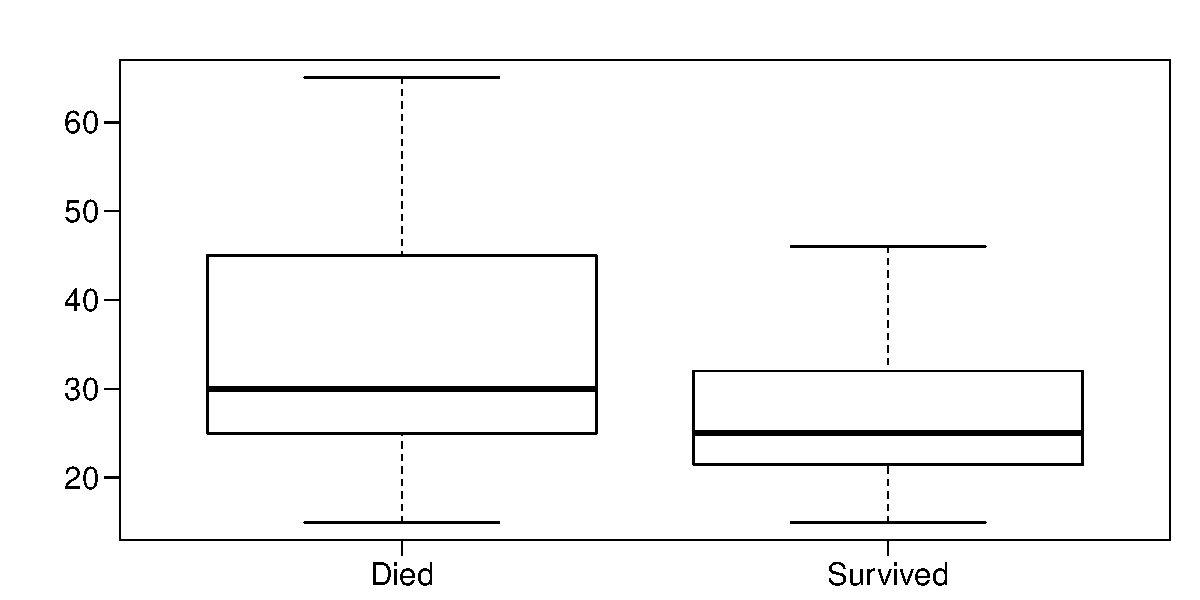
\includegraphics[width=0.8\textwidth]{9-5_logistic_reg/figures/donner/status_age}
\end{center}

\end{frame}

%%%%%%%%%%%%%%%%%%%%%%%%%%%%%%%%%%%

\begin{frame}
\frametitle{例 --- ドナー隊}

年齢と性別の両方が生存に影響を与えることは明らかだが、この関係を探るためのモデルをどのように作ればよいか？\\

~\\

死亡を 0、生存を 1 に設定しても、変換で解決できる問題ではない --- より高度な手法が必要である。

~\\

問題の捉え方の1つとして --- 生存と死亡を、確率が線形モデルの変換で与えられる二項分布から生じる成功と失敗として扱うことができる。

\end{frame}

%%%%%%%%%%%%%%%%%%%%%%%%%%%%%%%%%%%

\begin{frame}
\frametitle{一般化線形モデル}

これは回帰におけるこの種の問題に対処する非常に一般的な方法であり、結果として得られるモデルを一般化線形モデル（GLM）と呼ぶ。ロジスティック回帰はこのタイプのモデルの一例に過ぎない。\\
~\\
すべての一般化線形モデルは以下の3つの特性を持つ：
\begin{enumerate}
\item 応答変数を記述する確率分布
\item 線形モデル
\begin{itemize}
\item $\eta = \beta_0+\beta_1 X_1 + \cdots + \beta_n X_n$
\end{itemize}
\item 線形モデルと応答分布のパラメータを結びつけるリンク関数
\begin{itemize}
\item $g(p) = \eta$ または $p = g^{-1}(\eta)$
\end{itemize}
\end{enumerate}

\end{frame}

%%%%%%%%%%%%%%%%%%%%%%%%%%%%%%%%%%%

\subsection{ロジスティック回帰}

%%%%%%%%%%%%%%%%%%%%%%%%%%%%%%%%%%%

\begin{frame}
\frametitle{ロジスティック回帰}

ロジスティック回帰は、数値変数とカテゴリ変数の予測変数を用いて2値のカテゴリ応答変数をモデル化するための GLM である。\\
~\\
応答変数が二項分布から生じると仮定し、所与の予測変数セットに対する成功確率 $p$ をモデル化したい。\\
~\\

ロジスティックモデルの定式化を完成させるために、$\eta$ と $p$ を結びつける適切なリンク関数を設定する必要がある。様々な選択肢があるが、最もよく使われるのはロジット関数である。\\

~\\

\formula{ロジット関数}{
\[logit(p) = \log\left(\frac{p}{1-p}\right),\text{ ただし $0\le p \le 1$}\]
}

\end{frame}

%%%%%%%%%%%%%%%%%%%%%%%%%%%%%%%%%%%

\begin{frame}
\frametitle{ロジットの性質}

ロジット関数は 0 から 1 の間の値を取り、$-\infty$ から $\infty$ の値にマッピングする。\\
~\\

\formula{逆ロジット（ロジスティック）関数}
{
\[g^{-1}(x) = \frac{\exp(x)}{1+\exp(x)} = \frac{1}{1+\exp(-x)}\]
}

~\\
逆ロジット関数は $-\infty$ から $\infty$ の間の値を取り、0 から 1 の値にマッピングする。\\

~\\
この定式化はモデルの解釈にも有用で、ロジットは成功の対数オッズとして解釈できる（詳細は後述）。


\end{frame}

%%%%%%%%%%%%%%%%%%%%%%%%%%%%%%%%%%%

\begin{frame}
\frametitle{ロジスティック回帰モデル}

GLM の3つの基準から得られる：

\begin{align*}
y_i &\sim \text{Binom}(p_i)\\
\\
\eta &= \beta_0+\beta_1 x_1 + \cdots + \beta_n x_n\\
\\
\text{logit}(p) &= \eta
\end{align*}

ここから次の式が導かれる：

\[ p_i = \frac{\exp(\beta_0+\beta_1 x_{1,i} + \cdots + \beta_n x_{n,i})}{1+\exp(\beta_0+\beta_1 x_{1,i} + \cdots + \beta_n x_{n,i})} \]


\end{frame}

%%%%%%%%%%%%%%%%%%%%%%%%%%%%%%%%%%%

\begin{frame}[fragile]
\frametitle{例 --- ドナー隊 --- モデル}
\vspace{-2mm}
R では、\var{lm} の代わりに \var{glm} を使い、\var{family} 引数で適合する GLM の種類を指定することで、線形モデルと同様の方法で GLM を適合できる。\\

\vspace{2mm}

{\scriptsize
\begin{verbatim}
summary(glm(Status ~ Age, data=donner, family=binomial))

## Call:
## glm(formula = Status ~ Age, family = binomial, data = donner)
##
## Coefficients:
##             Estimate Std. Error z value Pr(>|z|)
## (Intercept)  1.81852    0.99937   1.820   0.0688 .
## Age         -0.06647    0.03222  -2.063   0.0391 *
##
##     Null deviance: 61.827  on 44  degrees of freedom
## Residual deviance: 56.291  on 43  degrees of freedom
## AIC: 60.291
##
## Number of Fisher Scoring iterations: 4
\end{verbatim}
}
\end{frame}


%%%%%%%%%%%%%%%%%%%%%%%%%%%%%%%%%%%

\begin{frame}
\frametitle{例 --- ドナー隊 --- 予測}

{\scriptsize
\begin{center}
\begin{tabular}{rrrrr}
  \hline
 & Estimate & Std. Error & z value & Pr($>$$|$z$|$) \\
  \hline
(Intercept) & 1.8185 & 0.9994 & 1.82 & 0.0688 \\
  Age & -0.0665 & 0.0322 & -2.06 & 0.0391 \\
   \hline
\end{tabular}
\end{center}
}

モデル：
\[\log\left(\frac{p}{1-p}\right) = 1.8185-0.0665\times \text{Age}\]

~\\~\\
新生児（Age=0）の生存オッズ/確率：
{\scriptsize
\begin{align*}
\log\left(\frac{p}{1-p}\right) &= 1.8185-0.0665\times \orange{0}\\
\frac{p}{1-p} &= \exp(1.8185) = 6.16 \\
p &= 6.16/7.16 = 0.86
\end{align*}
}

\end{frame}

%%%%%%%%%%%%%%%%%%%%%%%%%%%%%%%%%%%

\begin{frame}
\frametitle{例 --- ドナー隊 --- 予測（続き）}

モデル：
{\scriptsize
\[\log\left(\frac{p}{1-p}\right) = 1.8185-0.0665\times \text{Age}\]
}

25歳の生存オッズ/確率：
{\scriptsize
\begin{align*}
\log\left(\frac{p}{1-p}\right) &= 1.8185-0.0665\times \orange{25}\\
\frac{p}{1-p} &= \exp(0.156) = 1.17 \\
p &= 1.17/2.17 = 0.539
\end{align*}
}

50歳の生存オッズ/確率：
{\scriptsize
\begin{align*}
\log\left(\frac{p}{1-p}\right) &= 1.8185-0.0665\times \orange{50}\\
\frac{p}{1-p} &= \exp(-1.5065) = 0.222 \\
p &= 0.222/1.222 =  0.181
\end{align*}
}

\end{frame}

%%%%%%%%%%%%%%%%%%%%%%%%%%%%%%%%%%%

\begin{frame}
\frametitle{例 --- ドナー隊 --- 予測（続き）}

{\scriptsize
\[\log\left(\frac{p}{1-p}\right) = 1.8185-0.0665\times \text{Age}\]
}

\vspace{-10mm}

\begin{center}
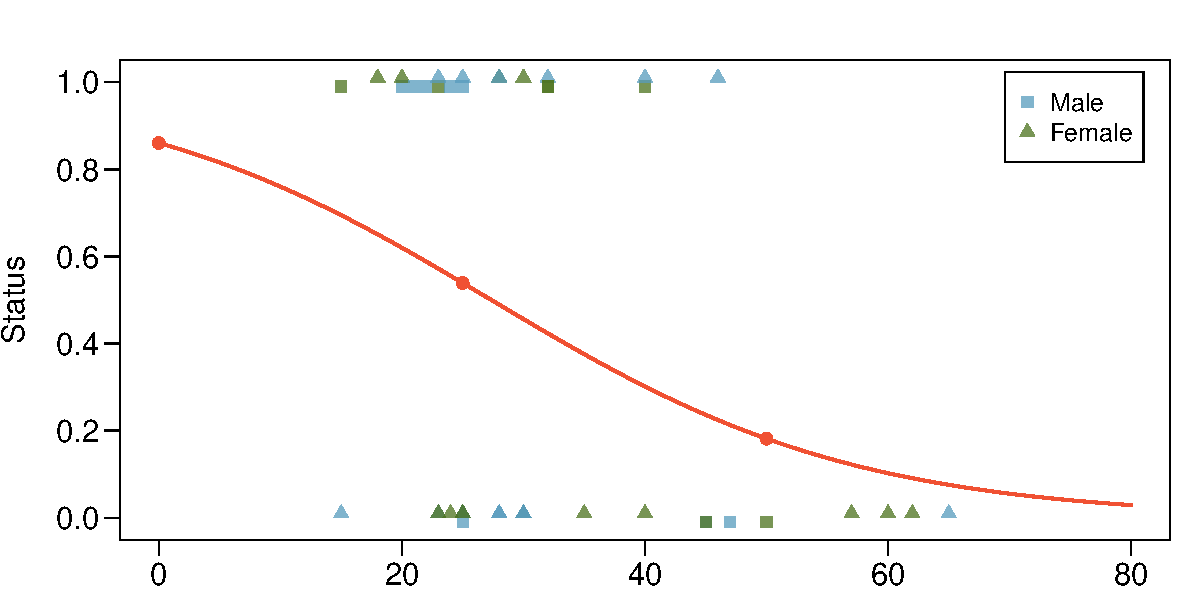
\includegraphics[width=0.8\textwidth]{9-5_logistic_reg/figures/donner/donner_scatter_pred.pdf}
\end{center}
\end{frame}

%%%%%%%%%%%%%%%%%%%%%%%%%%%%%%%%%%%

\begin{frame}
\frametitle{例 --- ドナー隊 --- 解釈}

{\scriptsize
\begin{center}
\begin{tabular}{rrrrr}
  \hline
 & Estimate & Std. Error & z value & Pr($>$$|$z$|$) \\
  \hline
(Intercept) & 1.8185 & 0.9994 & 1.82 & 0.0688 \\
  Age & -0.0665 & 0.0322 & -2.06 & 0.0391 \\
   \hline
\end{tabular}
\end{center}
}

単純な解釈は切片と傾きの項について、対数オッズと対数オッズ比の観点でのみ可能である。\\

~\\

\hl{切片}：年齢 0 のメンバーの生存の対数オッズ。ここからオッズや確率を計算できるが、追加計算が必要である。\\

~\\

\hl{傾き}：年齢が 1 単位増加する（1歳年上になる）と対数オッズ比がどれだけ変化するか。直感的には分かりにくい。多くの場合、符号と相対的な大きさのみを気にする。

\end{frame}

%%%%%%%%%%%%%%%%%%%%%%%%%%%%%%%%%%%

\begin{frame}[fragile]
\frametitle{例 --- ドナー隊 --- 解釈 --- 傾き}

{\scriptsize
\begin{align*}
\log\left(\frac{p_1}{1-p_1}\right) &= 1.8185-0.0665 (x+1) \\
                                   &= 1.8185-0.0665 x-0.0665 \\
\log\left(\frac{p_2}{1-p_2}\right) &= 1.8185-0.0665 x \\
\\
\log\left(\frac{p_1}{1-p_1}\right) - \log\left(\frac{p_2}{1-p_2}\right) &= -0.0665 \\
\log\left(\left. \frac{p_1}{1-p_1} \right/ \frac{p_2}{1-p_2} \right) &= -0.0665 \\
\left. \frac{p_1}{1-p_1} \right/ \frac{p_2}{1-p_2} &= \exp(-0.0665) = 0.94
\end{align*}
}

\end{frame}

%%%%%%%%%%%%%%%%%%%%%%%%%%%%%%%%%%%

\begin{frame}[fragile]
\frametitle{例 --- ドナー隊 --- 年齢と性別}
\vspace{-3mm}
{\tiny
\begin{verbatim}
summary(glm(Status ~ Age + Sex, data=donner, family=binomial))

## Call:
## glm(formula = Status ~ Age + Sex, family = binomial, data = donner)
##
## Coefficients:
##             Estimate Std. Error z value Pr(>|z|)
## (Intercept)  1.63312    1.11018   1.471   0.1413
## Age         -0.07820    0.03728  -2.097   0.0359 *
## SexFemale    1.59729    0.75547   2.114   0.0345 *
## ---
##
## (Dispersion parameter for binomial family taken to be 1)
##
##     Null deviance: 61.827  on 44  degrees of freedom
## Residual deviance: 51.256  on 42  degrees of freedom
## AIC: 57.256
##
## Number of Fisher Scoring iterations: 4
\end{verbatim}
}

\hl{性別の傾き}：他の予測変数を一定に保つとき、これは与えられた水準（Female）と参照水準（Male）の対数オッズ比である。

\end{frame}

%%%%%%%%%%%%%%%%%%%%%%%%%%%%%%%%%%%

\begin{frame}
\frametitle{例 --- ドナー隊 --- 性別別モデル}

重回帰と同様に、性別を代入することで男女それぞれの生存状況 vs. 年齢のモデルを得ることができる。\\
~\\

一般モデル：
{\scriptsize
\[\log\left(\frac{p_1}{1-p_1}\right) = 1.63312 + -0.07820\times\text{Age} + 1.59729\times\text{Sex}\]
}

男性モデル：
{\scriptsize
\begin{align*}
\log\left(\frac{p_1}{1-p_1}\right) &= 1.63312 + -0.07820\times\text{Age} + 1.59729\times\orange{0}\\
                                   &= 1.63312 + -0.07820\times\text{Age}
\end{align*}
}

女性モデル：
{\scriptsize
\begin{align*}
\log\left(\frac{p_1}{1-p_1}\right) &= 1.63312 + -0.07820\times\text{Age} + 1.59729\times\orange{1}\\
                                   &= 3.23041 + -0.07820\times\text{Age}
\end{align*}
}

\end{frame}

%%%%%%%%%%%%%%%%%%%%%%%%%%%%%%%%%%%

\begin{frame}
\frametitle{例 --- ドナー隊 --- 性別別モデル（続き）}

\begin{center}
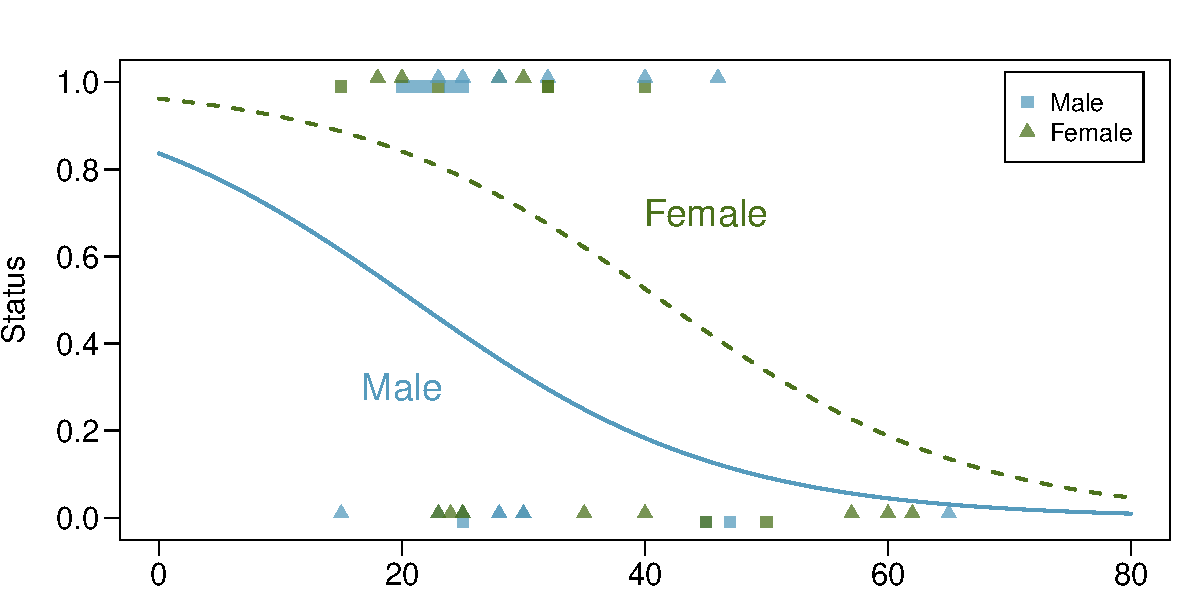
\includegraphics[width=\textwidth]{9-5_logistic_reg/figures/donner/donner_scatter_both.pdf}
\end{center}

\end{frame}

%%%%%%%%%%%%%%%%%%%%%%%%%%%%%%%%%%%

%%%%%%%%%%%%%%%%%%%%%%%%%%%%%%%%%%%

\begin{frame}[fragile,shrink]
\frametitle{モデル全体の仮説検定}
\vspace{-3mm}
{\scriptsize
\begin{verbatim}
summary(glm(Status ~ Age + Sex, data=donner, family=binomial))

## Call:
## glm(formula = Status ~ Age + Sex, family = binomial, data = donner)
##
## Coefficients:
##             Estimate Std. Error z value Pr(>|z|)
## (Intercept)  1.63312    1.11018   1.471   0.1413
## Age         -0.07820    0.03728  -2.097   0.0359 *
## SexFemale    1.59729    0.75547   2.114   0.0345 *
## ---
##
## (Dispersion parameter for binomial family taken to be 1)
##
##     Null deviance: 61.827  on 44  degrees of freedom
## Residual deviance: 51.256  on 42  degrees of freedom
## AIC: 57.256
##
## Number of Fisher Scoring iterations: 4
\end{verbatim}
}

\Note{モデル出力には F 統計量が含まれていない。一般的なルールとして、GLM モデルにはモデル全体の仮説検定が存在しない。}

\end{frame}

%%%%%%%%%%%%%%%%%%%%%%%%%%%%%%%%%%%

\begin{frame}
\frametitle{係数の仮説検定}

\begin{center}
\begin{tabular}{rrrrr}
  \hline
 & Estimate & Std. Error & z value & Pr($>$$|$z$|$) \\
  \hline
(Intercept) & 1.6331 & 1.1102 & 1.47 & 0.1413 \\
  Age & -0.0782 & 0.0373 & -2.10 & 0.0359 \\
  SexFemale & 1.5973 & 0.7555 & 2.11 & 0.0345 \\
   \hline
\end{tabular}
\end{center}

ただし、個々の係数についての推測は依然として可能であり、基本的な設定はこれまでに見てきたものとまったく同じだが、Z 検定を使用する。\\

~\\

\Note{唯一の難点は、このコースの範囲をはるかに超えるが、標準誤差の計算方法である。}

\end{frame}

%%%%%%%%%%%%%%%%%%%%%%%%%%%%%%%%%%%

\begin{frame}
\frametitle{年齢の傾き係数の検定}

{\small
\begin{center}
\begin{tabular}{rrrrr}
  \hline
            & Estimate & Std. Error & z value & Pr($>$$|$z$|$) \\
  \hline
(Intercept) & 1.6331  & 1.1102 & 1.47 & 0.1413 \\
        Age & \orange{-0.0782} & \green{0.0373} & \orange{-2.10} & \textcolor{blue}{0.0359} \\
  SexFemale & 1.5973  & 0.7555 & 2.11 & 0.0345 \\
   \hline
\end{tabular}
\end{center}
}

\begin{align*}
H_0:~& \beta_{age} = 0 \\
H_A:~& \beta_{age} \ne 0
\end{align*}

\begin{align*}
Z &= \frac{\hat{\beta_{age}} - \beta_{age}}{SE_{age}}
   = \frac{\orange{-0.0782} - 0}{\green{0.0373}} = \orange{-2.10} \\
\\
\text{p-value} &= P(|Z| > \orange{2.10}) = P(Z>\orange{2.10})+P(Z<\orange{-2.10})\\
               &= 2\times 0.0178 = \textcolor{blue}{0.0359}
\end{align*}

\end{frame}

%%%%%%%%%%%%%%%%%%%%%%%%%%%%%%%%%%%

%%%%%%%%%%%%%%%%%%%%%%%%%%%%%%%%%%%

\begin{frame}
\frametitle{年齢の傾き係数の信頼区間}

\begin{center}
\begin{tabular}{rrrrr}
  \hline
 & Estimate & Std. Error & z value & Pr($>$$|$z$|$) \\
  \hline
(Intercept) & 1.6331 & 1.1102 & 1.47 & 0.1413 \\
  Age & -0.0782 & 0.0373 & -2.10 & 0.0359 \\
  SexFemale & 1.5973 & 0.7555 & 2.11 & 0.0345 \\
   \hline
\end{tabular}
\end{center}

傾きの解釈は、予測変数の 1 単位の変化に対する対数オッズ比の変化であることを覚えておく。\\
~\\

対数オッズ比：
\[ CI = PE \pm CV \times SE = -0.0782 \pm 1.96 \times 0.0373 = (-0.1513,  -0.0051) \]

オッズ比：
\[ \exp(CI) = (\exp{-0.1513}, \exp{-0.0051}) = (0.8596,\ 0.9949) \]


\end{frame}


%%%%%%%%%%%%%%%%%%%%%%%%%%%%%%%%%%%

\subsection{追加例}

%%%%%%%%%%%%%%%%%%%%%%%%%%%%%%%%%%%


\begin{frame}
\frametitle{例 --- 野鳥飼育と肺がん}

1972〜1981年にオランダのハーグで実施された健康調査により、ペットの鳥の飼育と肺がんリスクの増加との関連が発見された。鳥の飼育をリスク因子として調査するために、研究者らは1985年にハーグ（人口45万人）の4つの病院で症例対照研究を実施した。彼らは一般開業医に登録されており、65歳以下で、1965年以降ハーグに居住していた患者の中から49例の肺がん症例を特定した。また、同じ年齢構成を持つ住民から98人の対照を選んだ。


\vfill

{\tiny From \textit{Ramsey, F.L. and Schafer, D.W. (2002). The Statistical Sleuth: A Course in Methods of Data Analysis (2nd ed)}}
\end{frame}

%%%%%%%%%%%%%%%%%%%%%%%%%%%%%%%%%%%

\begin{frame}
\frametitle{例 --- 野鳥飼育と肺がん --- データ}

{\scriptsize
\begin{tabular}{rllllrrr}
  \hline
    & \var{LC} & \var{FM} & \var{SS} & \var{BK} & \var{AG} & \var{YR} & \var{CD} \\
  \hline
  1 & LungCancer & Male & Low & Bird & 37.00 & 19.00 & 12.00 \\
  2 & LungCancer & Male & Low & Bird & 41.00 & 22.00 & 15.00 \\
  3 & LungCancer & Male & High & NoBird & 43.00 & 19.00 & 15.00 \\
\vdots & ~~~~~~\vdots & ~~~\vdots & ~~\vdots & ~~~\vdots & \vdots~~~ & \vdots~~~ & \vdots~~~ \\
147 & NoCancer & Female & Low & NoBird & 65.00 & 7.00 & 2.00 \\
   \hline
\end{tabular}
}

{\small
\begin{center}
\begin{tabular}{ll}
\var{LC} & 肺がんの有無 \\
\var{FM} & 対象者の性別 \\
\var{SS} & 社会経済的状況 \\
\var{BK} & 鳥の飼育の有無 \\
\var{AG} & 対象者の年齢（歳） \\
\var{YR} & 診断または検査前の喫煙年数 \\
\var{CD} & 平均喫煙率（1日当たりの本数）
\end{tabular}
\end{center}
}

\Note{NoCancer が参照応答（0 または失敗）、LungCancer が非参照応答（1 または成功）--- これは解釈に重要である。}

\end{frame}

%%%%%%%%%%%%%%%%%%%%%%%%%%%%%%%%%%%

\begin{frame}
\frametitle{例 --- 野鳥飼育と肺がん --- 探索的データ分析}

\begin{center}
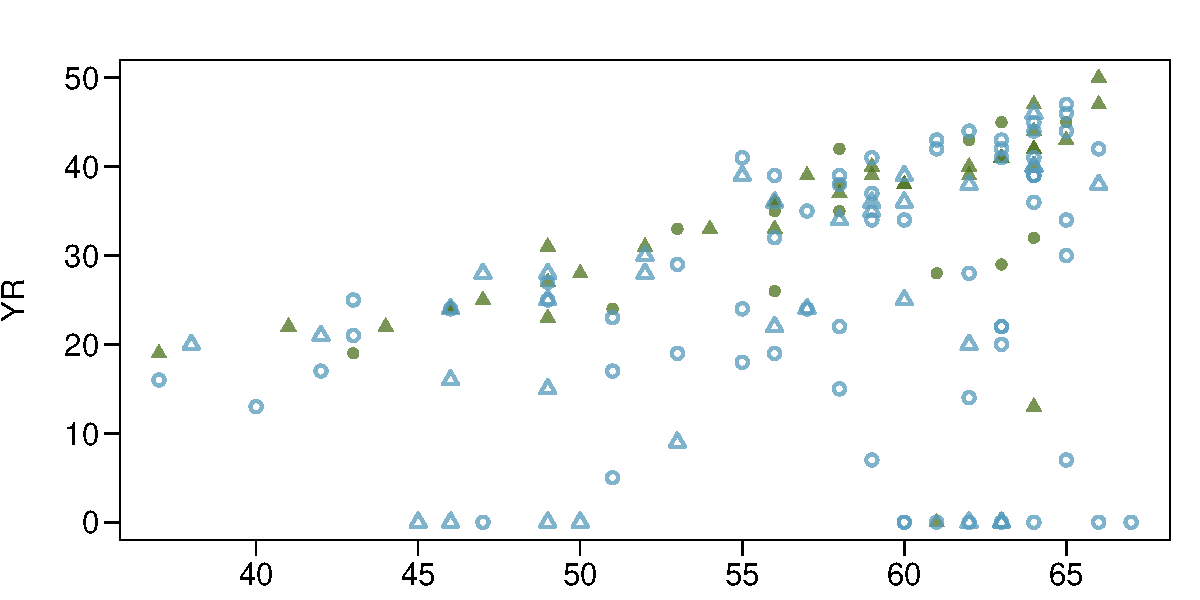
\includegraphics[width=0.8\textwidth]{9-5_logistic_reg/figures/birds/birds.pdf}
\end{center}

{\scriptsize
\begin{center}
\begin{tabular}{r|cc}
               & Bird（鳥あり）& No Bird（鳥なし）\\
\hline
Lung Cancer（肺がん）    & \textcolor{oiG}{$\blacktriangle$} & \textcolor{oiG}{$\bullet$} \\
No Lung Cancer（肺がんなし）& \textcolor{oiB}{$\triangle$}      & \textcolor{oiB}{$\circ$}
\end{tabular}
\end{center}
}



\end{frame}

%%%%%%%%%%%%%%%%%%%%%%%%%%%%%%%%%%%

\begin{frame}[fragile]
\frametitle{例 --- 野鳥飼育と肺がん --- モデル}

\vspace{-5mm}

{\tiny
\begin{verbatim}
summary(glm(LC ~ FM + SS + BK + AG + YR + CD, data=bird, family=binomial))

## Call:
## glm(formula = LC ~ FM + SS + BK + AG + YR + CD, family = binomial,
##     data = bird)
##
## Coefficients:
##             Estimate Std. Error z value Pr(>|z|)
## (Intercept) -1.93736    1.80425  -1.074 0.282924
## FMFemale     0.56127    0.53116   1.057 0.290653
## SSHigh       0.10545    0.46885   0.225 0.822050
## BKBird       1.36259    0.41128   3.313 0.000923 ***
## AG          -0.03976    0.03548  -1.120 0.262503
## YR           0.07287    0.02649   2.751 0.005940 **
## CD           0.02602    0.02552   1.019 0.308055
##
## (Dispersion parameter for binomial family taken to be 1)
##
##     Null deviance: 187.14  on 146  degrees of freedom
## Residual deviance: 154.20  on 140  degrees of freedom
## AIC: 168.2
##
## Number of Fisher Scoring iterations: 5
\end{verbatim}
}

\end{frame}

%%%%%%%%%%%%%%%%%%%%%%%%%%%%%%%%%%%

\begin{frame}
\frametitle{例 --- 野鳥飼育と肺がん --- 解釈}

\vspace{-5mm}

{\scriptsize
\begin{center}
\begin{tabular}{rrrrr}
  \hline
 & Estimate & Std. Error & z value & Pr($>$$|$z$|$) \\
  \hline
(Intercept) & -1.9374 & 1.8043 & -1.07 & 0.2829 \\
  FMFemale  & 0.5613 & 0.5312 & 1.06 & 0.2907 \\
  SSHigh    & 0.1054 & 0.4688 & 0.22 & 0.8221 \\
\rowcolor{gray}
  BKBird    & 1.3626 & 0.4113 & 3.31 & 0.0009 \\
  AG        & -0.0398 & 0.0355 & -1.12 & 0.2625 \\
\rowcolor{gray}
  YR        & 0.0729 & 0.0265 & 2.75 & 0.0059 \\
  CD        & 0.0260 & 0.0255 & 1.02 & 0.3081 \\
   \hline
\end{tabular}
\end{center}
}

他のすべての予測変数を一定に保つと、
\begin{itemize}
\item 鳥を飼育している人と飼育していない人の肺がんに関するオッズ比は $\exp(1.3626) = 3.91$ である。
\item 喫煙年数が 1 年増加することによる肺がんのオッズ比は $\exp(0.0729) = 1.08$ である。
\end{itemize}

\end{frame}

%%%%%%%%%%%%%%%%%%%%%%%%%%%%%%%%%%%

\begin{frame}
\frametitle{数値が意味しないこと ...}

ロジスティック回帰の解釈でよくある間違いは、オッズ比を確率の比として扱うことである。\\

~\\

鳥を飼育している人は、飼育していない人より肺がんを発症する可能性が 4 倍高いわけでは\emph{ない}。

~\\

これはリスク比とオッズ比の違いである。


\[RR = \frac{P(\text{疾患} | \text{曝露あり})}{P(\text{疾患} | \text{曝露なし})} \]

\[OR = \frac{P(\text{疾患} | \text{曝露あり}) / [1-P(\text{疾患} | \text{曝露あり})]}{P(\text{疾患} | \text{曝露なし})/[1-P(\text{疾患} | \text{曝露なし})]} \]


\end{frame}

%%%%%%%%%%%%%%%%%%%%%%%%%%%%%%%%%%%

\begin{frame}
\frametitle{鳥の話に戻る}

$P(\text{肺がん}|\text{鳥なし}) = 0.05$ とわかっている場合、鳥を飼育している人の肺がん確率は？

\begin{align*}
OR &= \frac{P(\text{肺がん} | \text{鳥あり}) / [1-P(\text{肺がん} | \text{鳥あり})]}{P(\text{肺がん} | \text{鳥なし})/[1-P(\text{肺がん} | \text{鳥なし})]} \\
\\
   &= \frac{P(\text{肺がん} | \text{鳥あり}) / [1-P(\text{肺がん} | \text{鳥あり})]}{0.05/[1-0.05]} = 3.91
\end{align*}

\[ P(\text{肺がん} | \text{鳥あり}) =  \frac{3.91 \times \frac{0.05}{0.95}}{1+3.91 \times \frac{0.05}{0.95}} = 0.171\]

\[ RR = P(\text{肺がん} | \text{鳥あり}) / P(\text{肺がん} | \text{鳥なし}) = 0.171 / 0.05 = 3.41\]

\end{frame}

%%%%%%%%%%%%%%%%%%%%%%%%%%%%%%%%%%

\begin{frame}
\frametitle{鳥の OR 曲線}

\vspace{-8mm}

\begin{center}
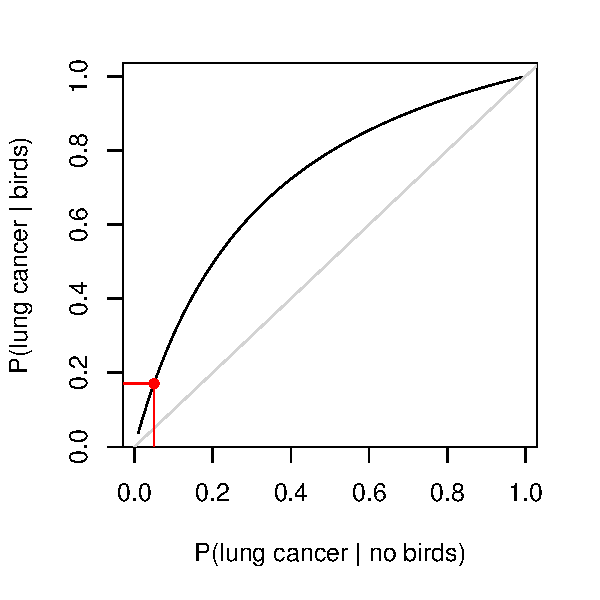
\includegraphics[width=0.7\textwidth]{9-5_logistic_reg/figures/birds/OR3.pdf}
\end{center}

\end{frame}

%%%%%%%%%%%%%%%%%%%%%%%%%%%%%%%%%%

\begin{frame}
\frametitle{OR 曲線}

\vspace{-5mm}

\begin{center}
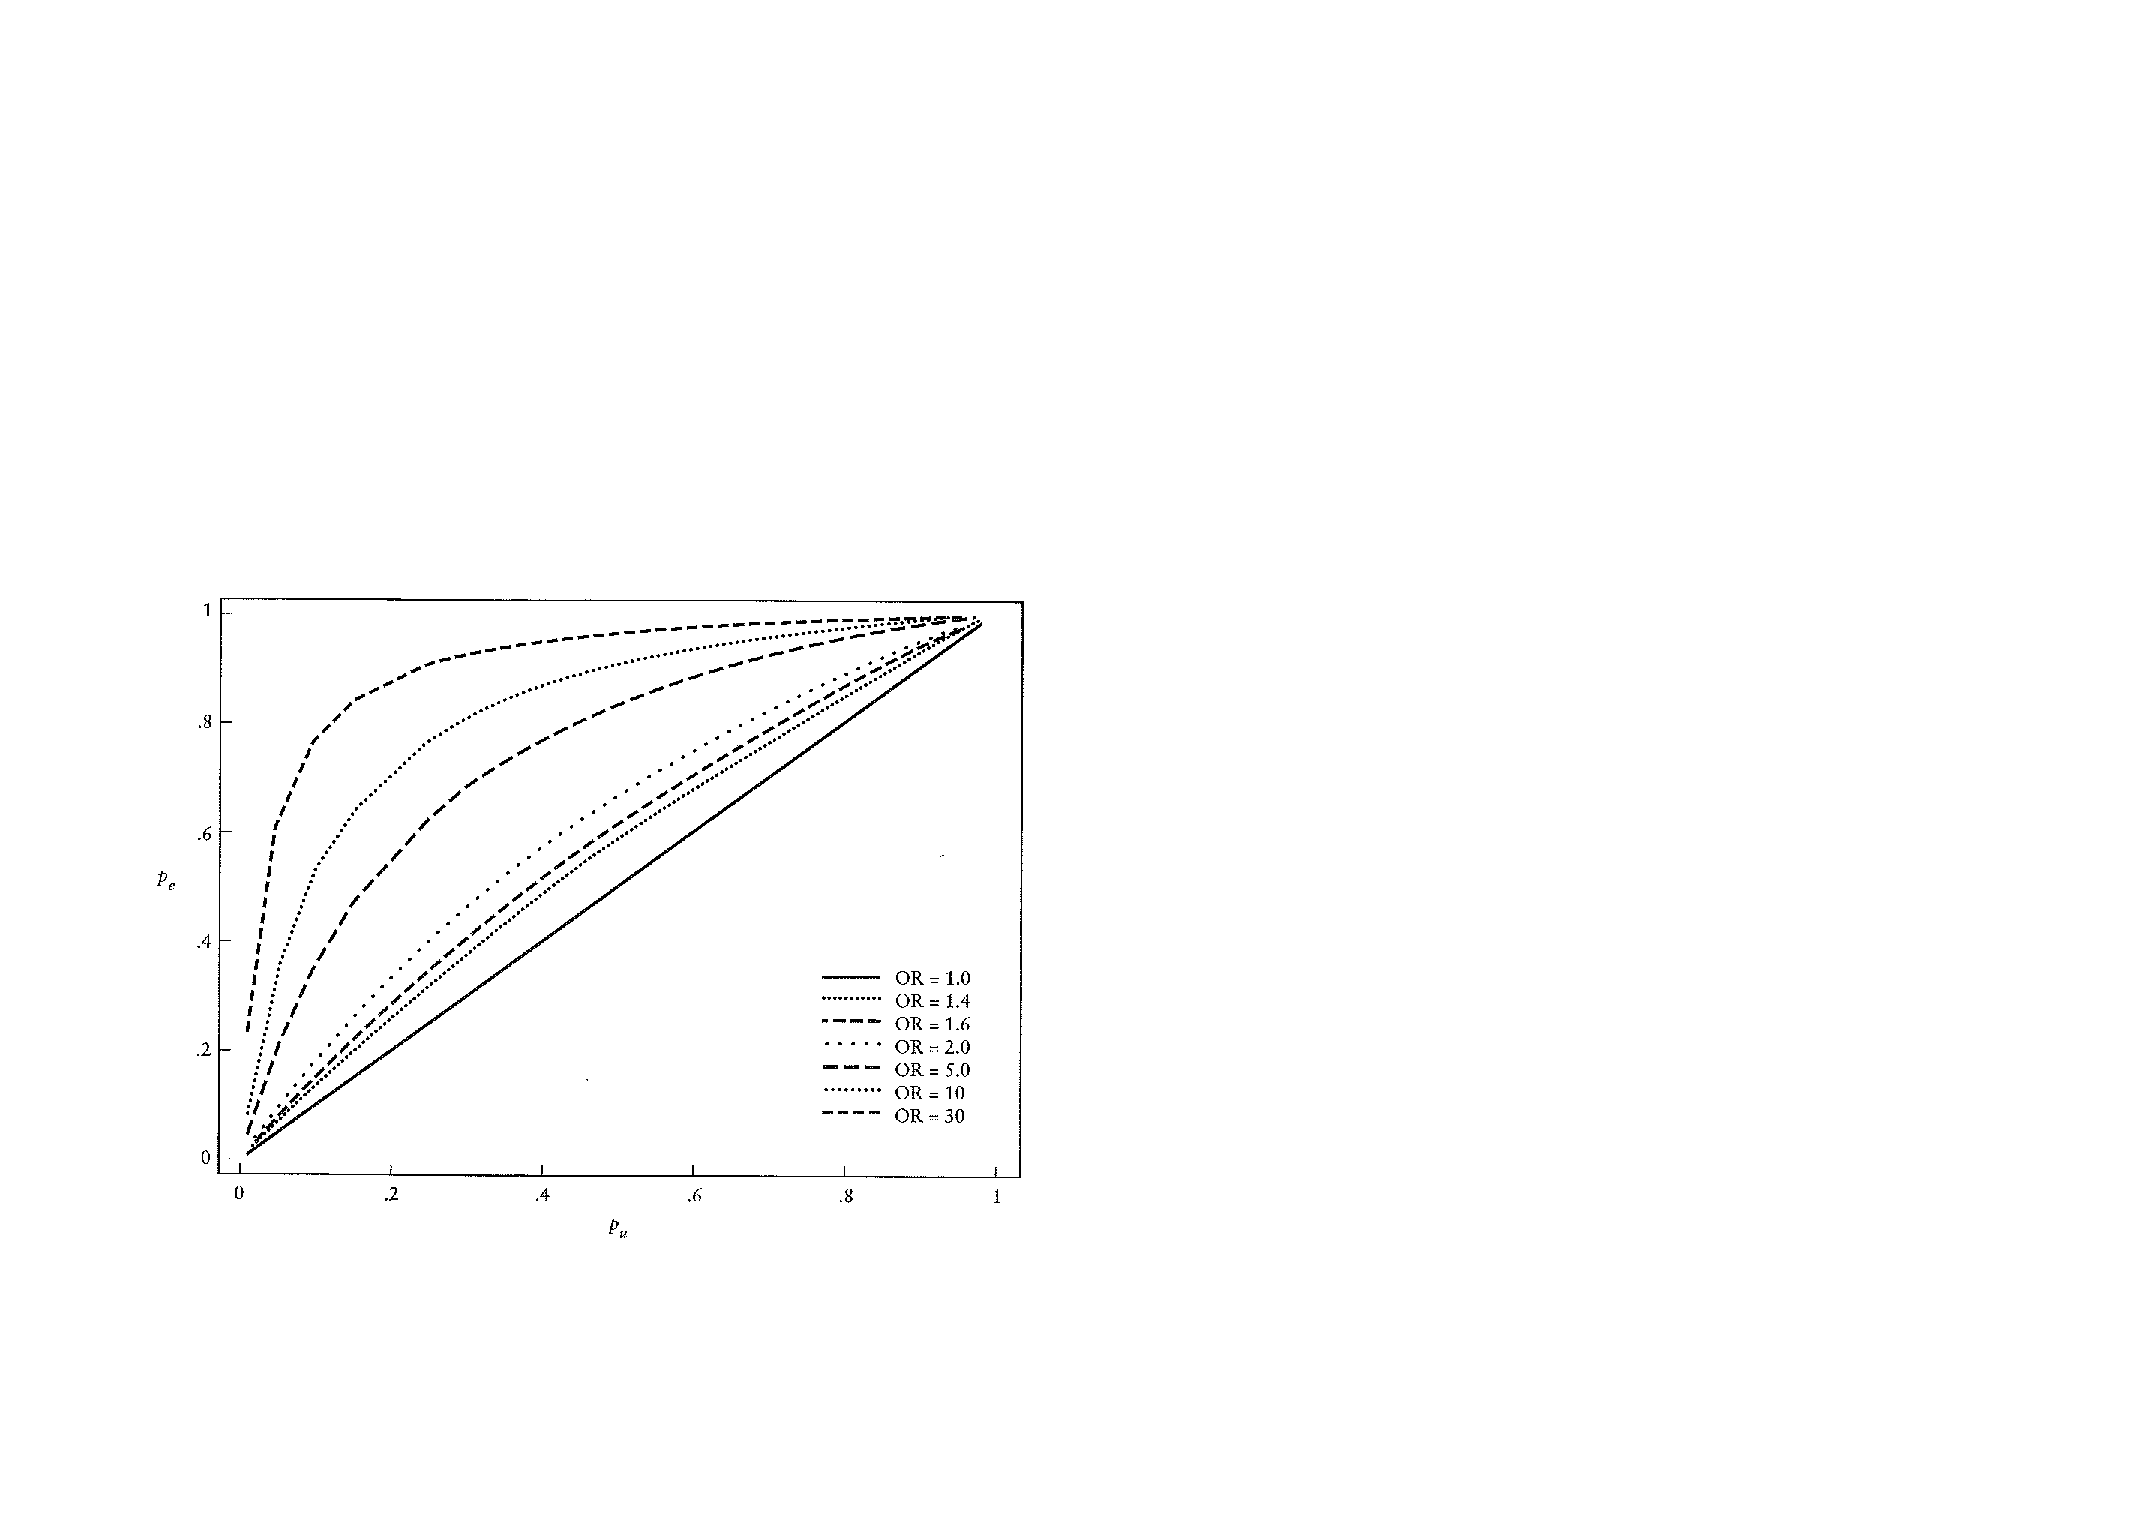
\includegraphics[width=0.85\textwidth]{9-5_logistic_reg/figures/all_OR.pdf}
\end{center}

\end{frame}

%%%%%%%%%%%%%%%%%%%%%%%%%%%%%%%%%%

\subsection{感度と特異度}

%%%%%%%%%%%%%%%%%%%%%%%%%%%%%%%%%%%

\begin{frame}
\frametitle{（昔の）例 --- \emph{House}}

Foxのテレビ番組 \emph{House} を見たことがあれば、House 医師が「ループスであることはない」とよく言うのを知っているだろう。\\
\vspace{3mm}
ループスは、外来細胞を攻撃して感染を防ぐはずの抗体が代わりに血漿タンパク質を外来物として認識し、血栓のリスクが高くなる医学的現象である。人口の 2\% がこの疾患に罹患していると考えられている。\\
\vspace{3mm}
ループスの検査は、実際にループスがある場合は非常に正確だが、ない場合は非常に不正確である。より具体的には、実際に疾患がある人に対して 98\% の精度を持つ。疾患がない人に対しては 74\% の精度を持つ。\\
\vspace{3mm}
ループスの検査が陽性であっても House 医師は正しいか？

\end{frame}

%%%%%%%%%%%%%%%%%%%%%%%%%%%%%%%%%%

\begin{frame}
\frametitle{（昔の）例 --- \emph{House}}

\begin{center}
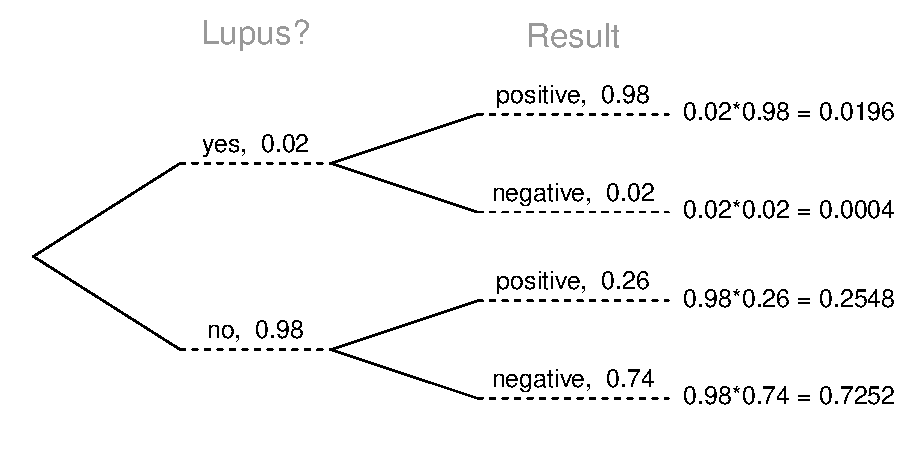
\includegraphics[width=0.8\textwidth]{9-5_logistic_reg/figures/tree_lupus.pdf}
\end{center}

{\footnotesize
\begin{align*}
P(\text{ループス} | +)  &= \frac{P(+,\text{ループス})}{P(+,\text{ループス})+P(+,\text{ループスなし})} \\
                     &= \frac{0.0196}{0.0196+0.2548} = 0.0714
\end{align*}
}
\end{frame}

%%%%%%%%%%%%%%%%%%%%%%%%%%%%%%%%%%

\begin{frame}
\frametitle{ループスの検査}
ループスの検査は実際には非常に複雑で、診断は通常、複数の検査結果に基づく。検査には全血球計算、赤血球沈降速度、腎臓・肝臓評価、尿検査、抗核抗体（ANA）検査などが含まれることが多い。\\
~\\
これらの各検査に何が関わるか（例えば全血球計算が高いか低いかの判断）と、個々の検査および関連する判断が患者へのループス診断の全体的な決定においてどのような役割を果たすかを考えることが重要である。\\

\end{frame}

%%%%%%%%%%%%%%%%%%%%%%%%%%%%%%%%%%

\begin{frame}
\frametitle{ループスの検査}

ある意味で、診断は様々な説明変数の複雑な統合を伴う二値決定（ループスかループスでないか）と見ることができる。\\
~\\
この例は診断がどのように行われるかについての情報を与えてくれないが、与えてくれる同様に重要なことがある --- それが検査の感度と特異度である。これらの値は陽性または陰性の検査結果が実際に何を意味するかを理解するために重要である。

\end{frame}

%%%%%%%%%%%%%%%%%%%%%%%%%%%%%%%%%%

\begin{frame}
\frametitle{感度と特異度}

\hl{感度（Sensitivity）} --- 検査が陽性結果を正しく識別する能力を測定する。
\[P(\text{検査}+~|~\text{疾患}+) = P(+ | \text{ループス}) = 0.98\]

\hl{特異度（Specificity）} --- 検査が陰性結果を正しく識別する能力を測定する。

\[P(\text{検査}-~|~\text{疾患}-) = P(- | \text{ループスなし}) = 0.74\]

\vspace{1cm}

極端なケースについて考えると理解が深まる --- 常に陽性を返す検査の感度と特異度は？常に陰性を返す検査は？

\end{frame}

%%%%%%%%%%%%%%%%%%%%%%%%%%%%%%%%%%

\begin{frame}
\frametitle{感度と特異度（続き）}

\vspace{-5mm}

\begin{center}
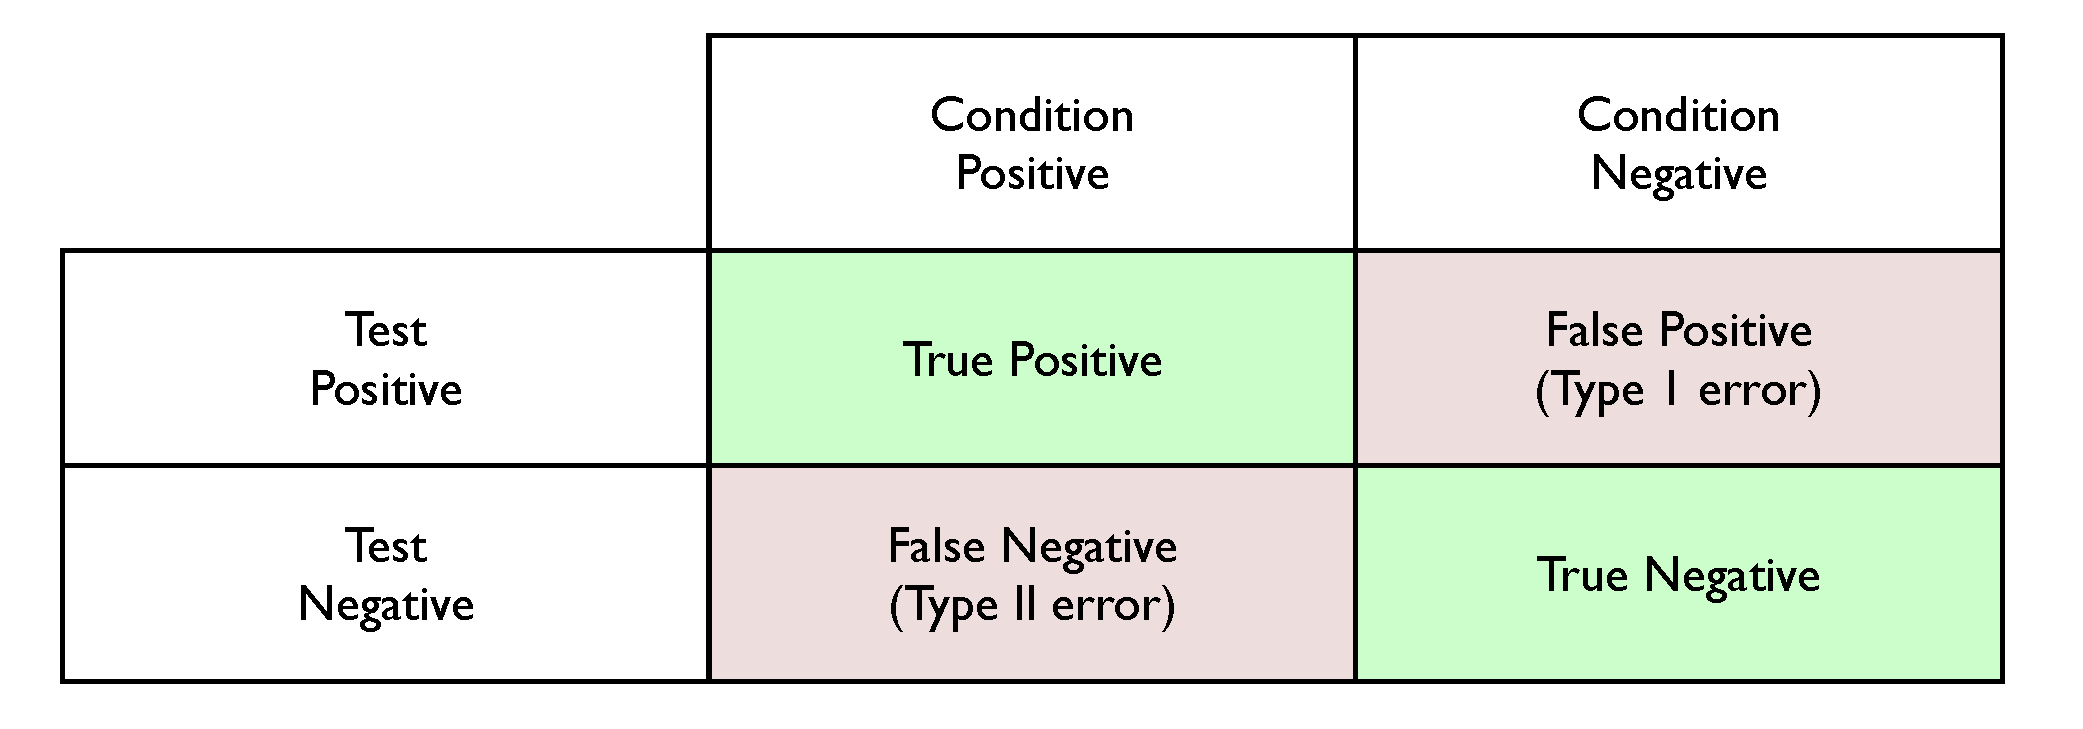
\includegraphics[width=\textwidth]{9-5_logistic_reg/figures/SenSpec.pdf}
\end{center}

\vspace{-9mm}

{\small
\begin{align*}
\text{\hl{感度}} &= P(\text{検査}+~|~\text{疾患}+) = TP / (TP + FN) \\
\text{\hl{特異度}} &= P(\text{検査}-~|~\text{疾患}-) = TN / (FP + TN)\\
\text{\hl{偽陰性率} (\hl{$\beta$})}  &= P(\text{検査}-~|~\text{疾患}+) = FN / (TP + FN) \\
\text{\hl{偽陽性率} (\hl{$\alpha$})} &= P(\text{検査}+~|~\text{疾患}-) = FP / (FP + TN)
\end{align*}

\vspace{-2mm}

\begin{align*}
\text{\hl{感度}} &= 1 - \text{\hl{偽陰性率}} = \text{検出力}\\
\text{\hl{特異度}} &= 1 - \text{\hl{偽陽性率}}
\end{align*}
}

\end{frame}

%%%%%%%%%%%%%%%%%%%%%%%%%%%%%%%%%%

\begin{frame}
\frametitle{それで？}

検査の感度と特異度（および/または偽陽性率と偽陰性率）を知ることが重要であることは明らかである。疾患の有病率（例：$P(\text{ループス})$）とともに、これらの値は $P(\text{ループス}|+)$ のような重要な量を計算するために必要である。\\
~\\
また、第1回中間試験前の検出力分析への簡単な取り組みも、偽陽性率と偽陰性率を最小化することに伴うトレードオフ（検出力を高めるには $\alpha$ または $n$ を増やす必要がある）について示唆を与えているはずである。\\
~\\
意思決定を行おうとするとき、この情報をどのように使うべきか？
\end{frame}

%%%%%%%%%%%%%%%%%%%%%%%%%%%%%%%%%%%

\subsection{ROC 曲線}

%%%%%%%%%%%%%%%%%%%%%%%%%%%%%%%%%%%

\begin{frame}
\frametitle{スパムに戻る}

今週の実験では、スパムメッセージを識別することに関心があるメールのデータセットを調べた。異なる予測変数がメッセージがスパムである確率にどう影響するかを評価するために、異なるロジスティック回帰モデルを検討した。\\

~\\

これらのモデルは受信メッセージに確率を割り当てるためにも使える（これは SLR / MLR の場合の予測に相当する）。しかし、スパムフィルターを設計するとしたら、これは半分の戦いに過ぎない。これらの確率を使って、どのメールをスパムとしてフラグを立てるかについての決定も行う必要がある。\\

~\\

唯一の解決策ではないが、閾値確率を選択し、その確率を超えたメールはスパムとしてフラグを立てるという単純なアプローチを考える。

\end{frame}


%%%%%%%%%%%%%%%%%%%%%%%%%%%%%%%%%%

\begin{frame}
\frametitle{閾値の選択}

\vspace{-5mm}

\begin{center}
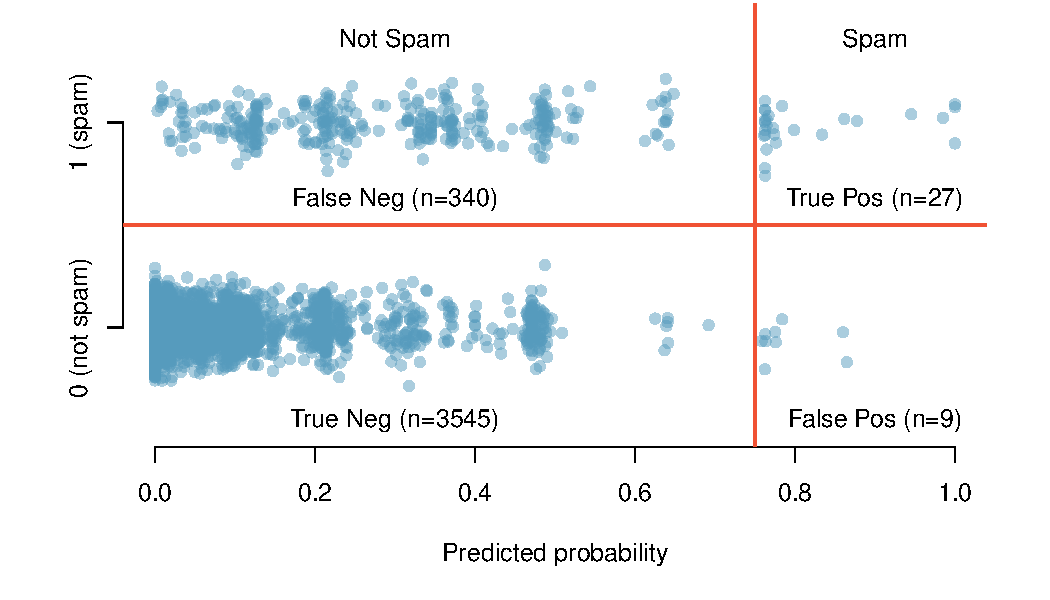
\includegraphics[width=\textwidth]{9-5_logistic_reg/figures/spam/spam5.pdf}
\end{center}

\vspace{-7mm}

\begin{center}
閾値を \orange{0.75} に設定した場合を見てみよう。
\end{center}

\end{frame}

%%%%%%%%%%%%%%%%%%%%%%%%%%%%%%%%%%

\begin{frame}
\frametitle{閾値選択の結果}

メールデータセットで閾値 0.75 を選ぶと以下の結果が得られる：
\vspace{-1.5mm}
\begin{align*}
FN = 340 &\qquad TP = 27 \\
TN = 3545 &\qquad FP = 9
\end{align*}

この意思決定ルールの感度と特異度は？

\soln{
\begin{align*}
\text{感度} & = TP / (TP + FN) = 27 / (27+340) = 0.073 \\
\text{特異度} & = TN / (FP + TN) = 3545 / (9+3545) = 0.997 \\
\end{align*}
}

\end{frame}

%%%%%%%%%%%%%%%%%%%%%%%%%%%%%%%%%%

\begin{frame}
\frametitle{他の閾値を試す}

\vspace{-5mm}

\begin{center}
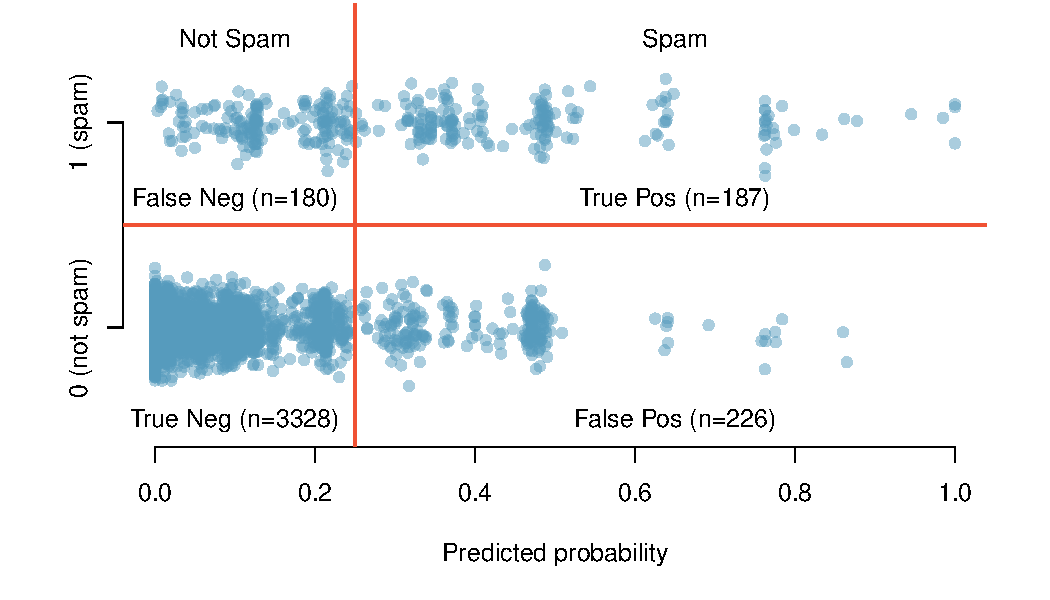
\includegraphics[width=0.9\textwidth]{9-5_logistic_reg/figures/spam/spam5-5.pdf}
\end{center}

{\footnotesize
\begin{center}
\begin{tabular}{|c|ccccc|}
\hline
閾値   & 0.75 & 0.625 & 0.5 & 0.375 & 0.25 \\
\hline
感度 & 0.074 & 0.106 & 0.136 & 0.305 & 0.510 \\
特異度 & 0.997 & 0.995 & 0.995 & 0.963 & 0.936 \\
\hline
\end{tabular}
\end{center}
}

\end{frame}


%%%%%%%%%%%%%%%%%%%%%%%%%%%%%%%%%%

\begin{frame}
\frametitle{感度と特異度の関係}

{\footnotesize
\begin{center}
\begin{tabular}{|c|ccccc|}
\hline
閾値   & 0.75 & 0.625 & 0.5 & 0.375 & 0.25 \\
\hline
感度 & 0.074 & 0.106 & 0.136 & 0.305 & 0.510 \\
特異度 & 0.997 & 0.995 & 0.995 & 0.963 & 0.936 \\
\hline
\end{tabular}
\end{center}
}


\begin{center}
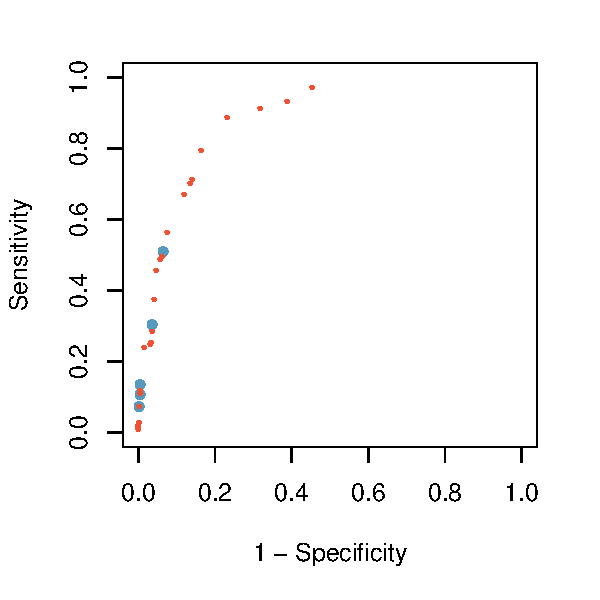
\includegraphics[width=0.5\textwidth]{9-5_logistic_reg/figures/spam/sen_vs_spec3.pdf}
\end{center}

\end{frame}

%%%%%%%%%%%%%%%%%%%%%%%%%%%%%%%%%%

\begin{frame}
\frametitle{受信者操作特性（ROC）曲線}

\vspace{-8mm}

\begin{center}
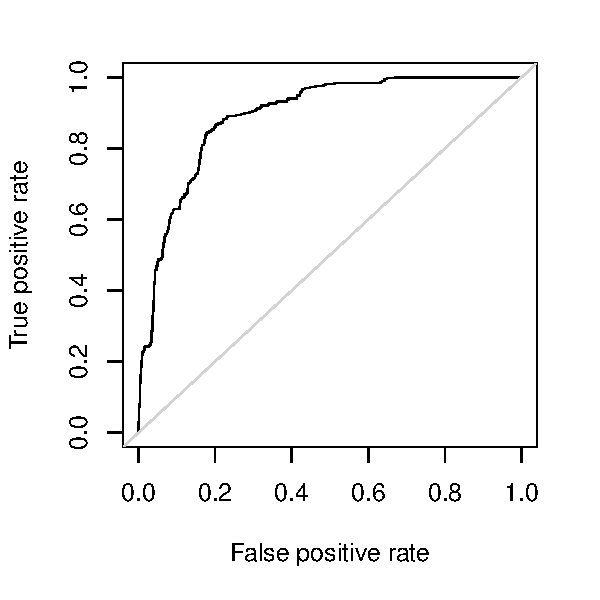
\includegraphics[width=0.7\textwidth]{9-5_logistic_reg/figures/spam/ROC.pdf}
\end{center}

\end{frame}

%%%%%%%%%%%%%%%%%%%%%%%%%%%%%%%%%%

\begin{frame}
\frametitle{受信者操作特性（ROC）曲線（続き）}

なぜ ROC 曲線を使うのか？

\begin{itemize}
\item すべての可能な閾値における感度と特異度のトレードオフを示す。

\item 偶然による性能との比較が直感的にわかる。

\item 曲線下面積（AUC）をモデルの予測能力の評価として使用できる。

\end{itemize}

\end{frame}

%%%%%%%%%%%%%%%%%%%%%%%%%%%%%%%%%%

\begin{frame}[fragile]
\frametitle{スパムモデルの精緻化}

\vspace{-5mm}

{\footnotesize
\begin{verbatim}
g_refined = glm(spam ~ to_multiple+cc+image+attach+winner
                      +password+line_breaks+format+re_subj
                      +urgent_subj+exclaim_mess,
                data=email, family=binomial)
summary(g_refined)
\end{verbatim}

\begin{center}
\begin{tabular}{rrrrr}
  \hline
 & Estimate & Std. Error & z value & Pr($>$$|$z$|$) \\
  \hline
(Intercept) & -1.7594 & 0.1177 & -14.94 & 0.0000 \\
  to\_multipleyes & -2.7368 & 0.3156 & -8.67 & 0.0000 \\
  ccyes & -0.5358 & 0.3143 & -1.71 & 0.0882 \\
  imageyes & -1.8585 & 0.7701 & -2.41 & 0.0158 \\
  attachyes & 1.2002 & 0.2391 & 5.02 & 0.0000 \\
  winneryes & 2.0433 & 0.3528 & 5.79 & 0.0000 \\
  passwordyes & -1.5618 & 0.5354 & -2.92 & 0.0035 \\
  line\_breaks & -0.0031 & 0.0005 & -6.33 & 0.0000 \\
  formatPlain & 1.0130 & 0.1380 & 7.34 & 0.0000 \\
  re\_subjyes & -2.9935 & 0.3778 & -7.92 & 0.0000 \\
  urgent\_subjyes & 3.8830 & 1.0054 & 3.86 & 0.0001 \\
  exclaim\_mess & 0.0093 & 0.0016 & 5.71 & 0.0000 \\
   \hline
\end{tabular}
\end{center}

}
\end{frame}

%%%%%%%%%%%%%%%%%%%%%%%%%%%%%%%%%%

\begin{frame}[fragile]
\frametitle{モデルの比較}

\vspace{-8mm}

\begin{center}
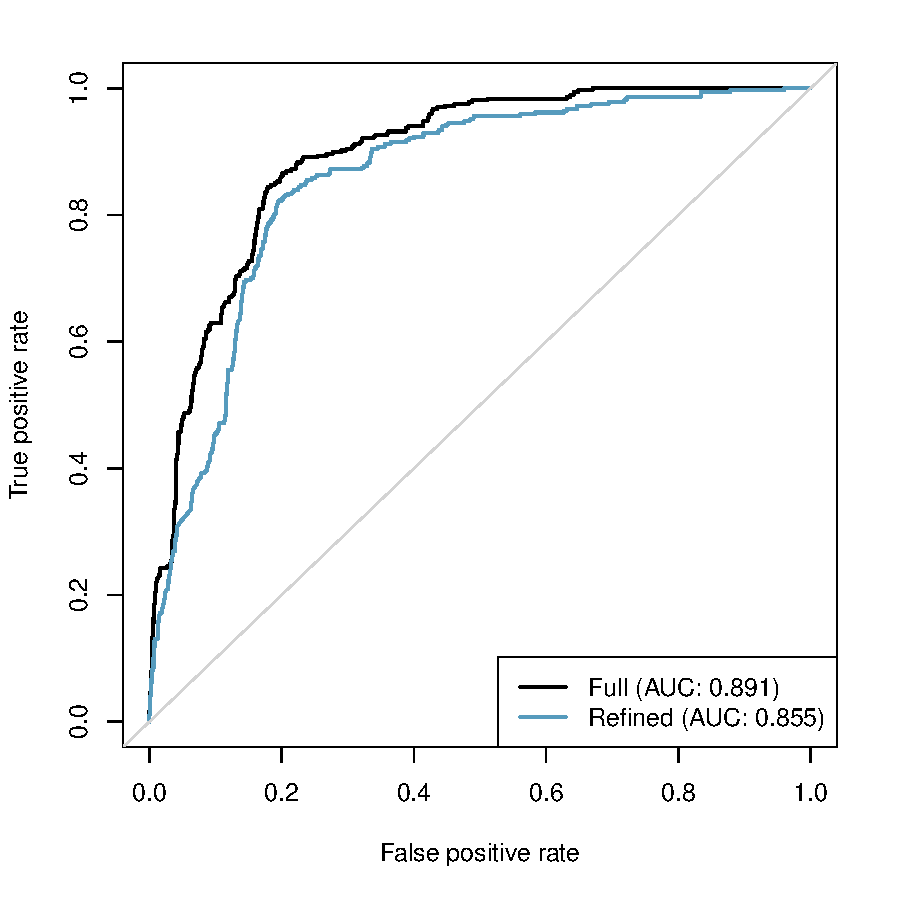
\includegraphics[width=0.7\textwidth]{9-5_logistic_reg/figures/spam/ROC_comp.pdf}
\end{center}

\end{frame}

%%%%%%%%%%%%%%%%%%%%%%%%%%%%%%%%%%

\subsection{効用関数}

%%%%%%%%%%%%%%%%%%%%%%%%%%%%%%%%%%%

\begin{frame}
\frametitle{効用関数}

「最良の」閾値を決定するために使える合理的な定量的アプローチは他にも多くある。\\
~\\
経済学のコースを受けたことがあれば、効用関数のアイデアを聞いたことがあるだろう。各結果に対してコストと利益を割り当て、各状況の効用を計算するためにそれらを使うことができる。

\end{frame}

%%%%%%%%%%%%%%%%%%%%%%%%%%%%%%%%%%

\begin{frame}
\frametitle{スパムフィルターの効用関数}

スパムフィルターの効用関数を記述するには、各結果のコスト/利益を考慮する必要がある。

\begin{center}
 \renewcommand\arraystretch{1.5}
\begin{tabular}{l|c}
結果 & 効用 \\
\hline
真陽性（TP）  & 1 \\
真陰性（TN）  & 1 \\
偽陽性（FP） & -50 \\
偽陰性（FN） & -5 \\
\end{tabular}
\end{center}
~\\
\[U(p) = TP(p) + TN(p) - 50 \times FP(p) - 5 \times FN(p)\]

\end{frame}

%%%%%%%%%%%%%%%%%%%%%%%%%%%%%%%%%%

\begin{frame}
\frametitle{閾値 0.75 の効用}

メールデータセットで閾値 0.75 を選ぶと以下の結果が得られる：
\vspace{-1.5mm}
\begin{align*}
FN = 340 &\qquad TP = 27 \\
TN = 3545 &\qquad FP = 9
\end{align*}

\begin{align*}
U(p) &= TP(p) + TN(p) - 50 \times FP(p) - 5 \times FN(p) \\
     &= 27+3545-50\times9-5\times340 = 1422
\end{align*}

それ自体では有用ではないが、他の閾値と比較することができる。

\end{frame}

%%%%%%%%%%%%%%%%%%%%%%%%%%%%%%%%%%

\begin{frame}
\frametitle{効用曲線}

\vspace{-5mm}

\begin{center}
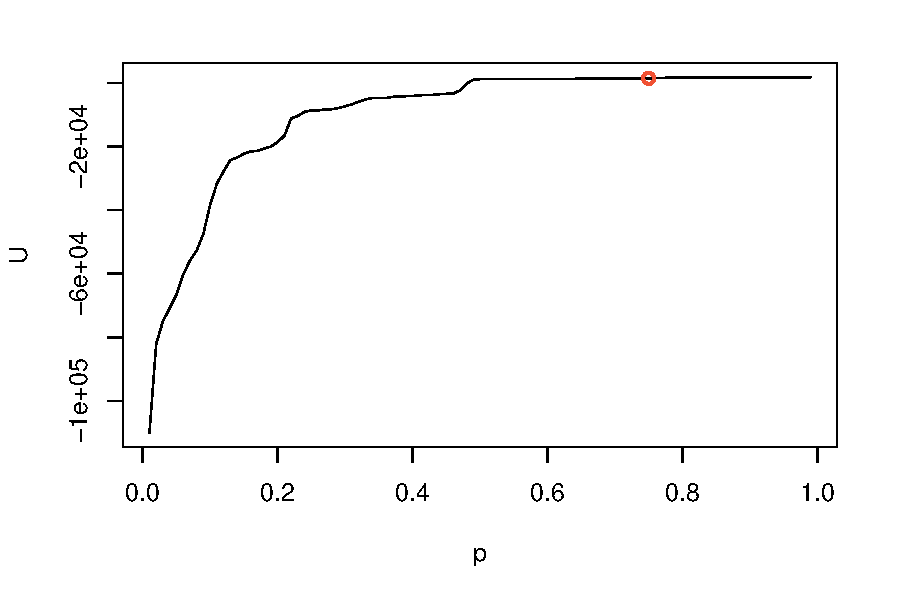
\includegraphics[width=\textwidth]{9-5_logistic_reg/figures/spam/utility.pdf}
\end{center}

\end{frame}


%%%%%%%%%%%%%%%%%%%%%%%%%%%%%%%%%%

\begin{frame}
\frametitle{効用曲線（拡大）}

\vspace{-5mm}

\begin{center}
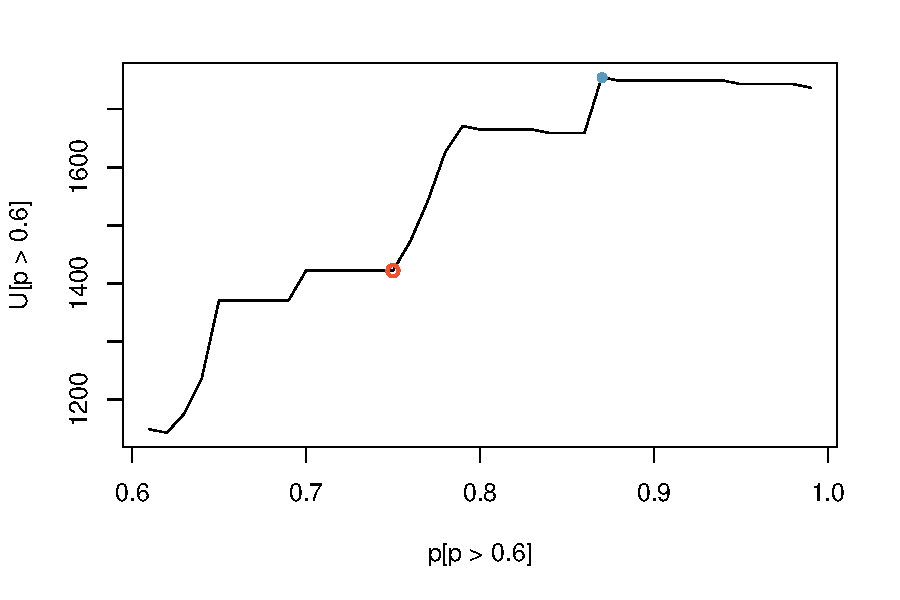
\includegraphics[width=\textwidth]{9-5_logistic_reg/figures/spam/utility3.pdf}
\end{center}

\end{frame}

%%%%%%%%%%%%%%%%%%%%%%%%%%%%%%%%%%

\begin{frame}
\frametitle{最大効用}

\begin{center}
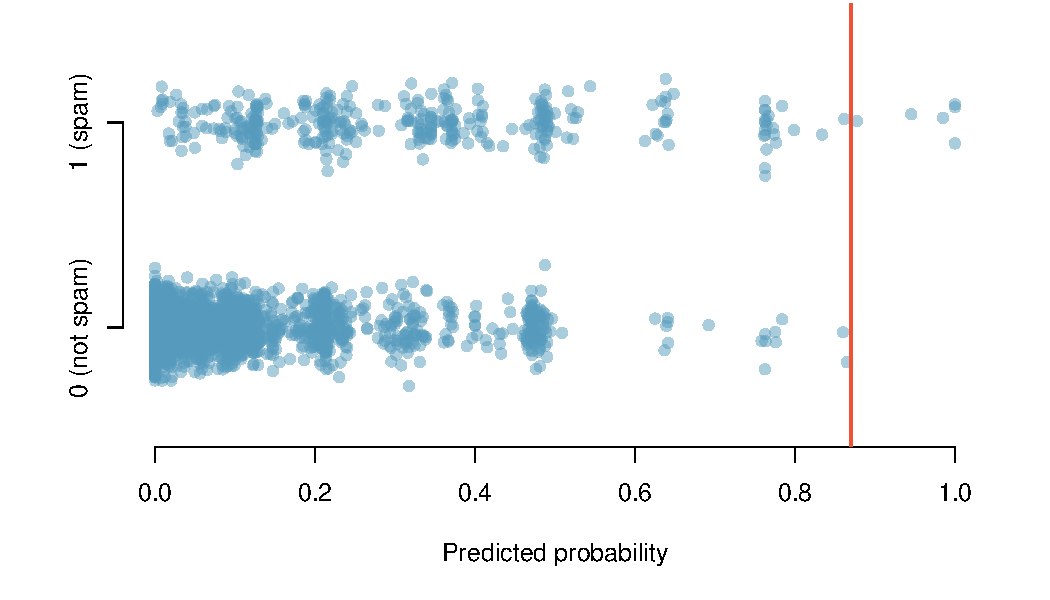
\includegraphics[width=\textwidth]{9-5_logistic_reg/figures/spam/utility4.pdf}
\end{center}

\end{frame}



%%%%%%%%%%%%%%%%%%%%%%%%%%%%%%%%%%%%
% ドキュメント終了
%%%%%%%%%%%%%%%%%%%%%%%%%%%%%%%%%%%%

\end{document}
